%%
%% Qbe SAS SystemDocumentation
%%     special edition for htl
%% (C) Copyright 2001-2004 Christian Hofstaedtler
%%
%% $Id$
%%
\documentclass[a4paper,11pt,oneside]{book}

\newcommand{\ionusdocdate}{\today}
\newcommand{\ionusdoctitle}{Qbe SAS}
\newcommand{\ionusdocauthor}{Christian\ Hofst�dtler}

\usepackage[latin1]{inputenc}
\usepackage[T1]{fontenc}

\usepackage{ngerman,color,latexsym,alltt}
\usepackage{graphics}
\usepackage[pdftex]{graphicx}
\usepackage[pdftex,plainpages=false]{hyperref}
\usepackage[ngerman]{babel}
% Packages
\usepackage{listings}
\usepackage{fancyhdr}
\usepackage{fancyvrb}
\usepackage{longtable}
\usepackage{url}
\usepackage{multicol}

\usepackage{pdfpages}
\usepackage{pdflscape}

\usepackage{geometry}
\usepackage{calc}

\usepackage{makeidx}
\usepackage{doxygen}
\makeindex

%% HyperRef
\hypersetup{%
	pdftitle = {\ionusdoctitle},
	pdfauthor = {\textcopyright\ \ionusdocauthor},
	pdfcreator = {\LaTeX\ with package \flqq hyperref\frqq},
	pdfborder = 0,
	pdfstartpage = 1,
	bookmarks = true,
	bookmarksopen = true,
}

\newcommand{\placefig}[2]{%
\begin{figure}[h] %
	\centering % 
		\includegraphics{files/#1} %
		\caption{#2} %
	\label{fig:#1} %
\end{figure} %
}

\newcommand{\placefigx}[3]{%
\begin{figure}[h] %
	\centering %
		\includegraphics[#3]{files/#1} %
		\caption{#2} %
	\label{fig:#1} %
\end{figure} %
}

%\definecolor{Headings}{rgb}{1,0,0}%{named}{Red}
%\newcommand{\cChapter}[1]{\color{Headings}\chapter{#1}\color{black}}
\newcommand{\cChapter}[1]{\chapter{#1}}


\renewcommand*\descriptionlabel[1]{\hspace\labelsep
	\color{red}\bfseries #1\hspace{4pt} }


%fontfamily=Helvetica,
%\fvset{frame=single,fontsize=\small,numbers=left,numbersep=3pt}

\definecolor{identifiers}{rgb}{0.1,0.1,0.1}

\lstset{% listings setup
	basicstyle=\small,%
	numbers=left,numberstyle=\tiny,stepnumber=1,numbersep=5pt,%
	tabsize=4,%
%       frame=single,%
	breaklines=true,%
	language=C,%
	showstringspaces=false,showspaces=false,showtabs=false,%
	keywordstyle=\color{blue},commentstyle=\color{green},identifierstyle=\color{identifiers}%
}

% Bookmarks fixup
\ifx\hypersetup\undefined\else
\pdfstringdefDisableCommands{\renewcommand{\color}[1]{}}%
\pdfstringdefDisableCommands{\edef\ci{\textbackslash}}%
\pdfstringdefDisableCommands{\edef\sim{\textasciitilde}}%
\pdfstringdefDisableCommands{\edef\circ{\textdegree}}%
\pdfstringdefDisableCommands{\edef\ldots{... }}%
\fi




\nonfrenchspacing

\begin{document}
\pagenumbering{roman}

% Set Document Information
\date{\ionusdocdate}
\author{\ionusdocauthor}
\title{\ionusdoctitle}


\begin{titlepage}
{
\nonfrenchspacing
\begin{center}
HTBLuVA Wiener Neustadt \\
\rule{\textwidth}{0.5pt}
ABTEILUNG f�r ELEKTROTECHNIK \\
Industrielle Elektronik / Informationstechnik \\

\vspace{2cm}

Diplomarbeit / Abschlussarbeit \\
\normalsize

\vspace{1cm}

\Huge%
Redundantes LAN-Anmelde- und Verwaltungssystem \\
\normalsize

\vspace{3.5cm}

von \\

\vspace{1cm}

Christian Hofst�dtler \\

\vspace{3cm}

\textbf{Begutachter: Dr. K. Filz} \\

\vfill

Wiener Neustadt, Juni 2004
\medskip

\par
\end{center}
}
\end{titlepage}

\fontfamily{cmbr}
\selectfont

%%% Preflight pages
\pagestyle{empty}
\normalsize

\newpage	%% Copyright, Thanks
\noindent Dokumentation Copyright \copyright  2001, 2002, 2003, 2004 Christian Hofst�dtler. 

\vspace{2cm}

\noindent Irrt�mer, Druck- und Tippfehler sowie �berm�dung vorbehalten. \\ 
Rechtschreib- und Grammatikfehler im Preis inbegriffen.

\vspace{5cm}

\noindent Typesetter: pdf\LaTeXe with HyperRef.

\noindent Datei kompiliert: \today.


\newpage
{
\begin{center}
\vspace{6cm} 

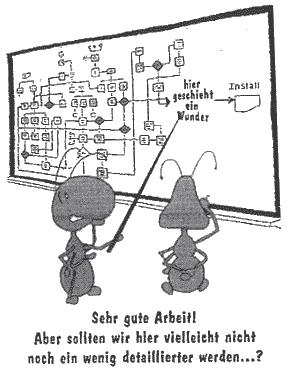
\includegraphics{files/projekt_wunder} \\ 
\medskip
\textit{F�r den Weg den ich hier beschritten habe. Dies ist das einzige was diesen Weg rechtfertigt und die Hoffnung transportiert, dass dies jemals jemand anderer verstehen w�rde.}
\end{center}
}


\pagestyle{plain}

\normalsize
\newpage
\tableofcontents

%\newpage
%\listoffigures															      

\newpage

%\cChapter{Allgemein}
\subsection*{Abstrakt}

Dieses Projekt entstand aus der schier unm�glichen Aufgabe, 1500 Sch�lern den Zugriff auf ein neues HTL-Netzwerk sowie das Internet zu geben -- mit m�glichst wenig Geld, und keinem zus�tzlichen Verwaltungsaufwand. Dass dies so nicht funktionieren w�rde, war von Anfang an klar, jedoch konnte man immer noch versuchen, den neuen Verwaltungsaufwand m�glichst gering zu halten. Damit war das Ziel klar: neue Systeme, mit neuer Software mussten beschafft werden, um diese 1500 Benutzer zentral so verwaltbar zu machen, dass dies eine Person neben der normalen Lehrverpflichtung schaffen kann.

W�hrend der 3 Jahre des Projektaufbaus, kamen immer neue Anforderungen hinzu und neue Systeme (Informationssystem, Wetterstation, Inventarverwaltung) mussten eingebunden werden.

\medskip

Einige dieser neuen Systeme, und auch dieses Projekt, finden sich nunmehr unter dem Titel Qbe Systems wieder.

\subsection*{Abstract}

This project claims to provide a full featured network administration for about 1500 users. 
Started with about zero money, a short time frame and the ultimate goal to not add any more administrative tasks, so it was clear to start with the best -- Open Source.

\medskip

While the project evolved over three years, new goals were added and it was required that other systems like EIV\footnote{Electronic Inventory Acquisition and Administration} were easy to integrate. Some of these new systems are now part of the Qbe family.


\subsection{State of the Art}
Dieses Projekt basiert auf der modernen Debian GNU/Linux\footnote{\url{http://www.debian.org/} } Distribution als Betriebssystem, dem welt-besten Verzeichnisdienst Novell eDirectory \footnote{\url{http://www.novell.com/edirectory/} } und von Grund auf neu geschriebener Benutzerverwaltungs- und Client-Software. 
Damit wird auf fundierte Internet-Standards wie HTTP\footnote{HyperText Transmission Protocol}, LDAP\footnote{Lightweight Directory Access Protocol} und RPC\footnote{Remote Procedure Call}, die heute als zukunftsweisend gelten, gebaut.



\subsection*{�ber den Autor}

Als Einzelprojektant war es nicht immer leicht dieses Projekt komplett durchzuziehen. M�glich schon gar nicht, Hilfe habe ich von einigen Seiten erhalten. Trotzdem hat dieses Projekt genug Spuren hinterlassen und Erfahrungen gebracht. \\


\subsubsection*{Dank ...}

\vspace{1.3cm}

\noindent \textit{Dank spricht man nicht aus,} \\
\noindent \textit{sondern man schreibt ihn auf.} \\

\vspace{1.3cm}

\begin{description}

\item{Dr. Karl Filz} \\ 
	Professioneller Projektleiter und Ratgeber

\item{Andreas St�tzner} \\ 
	Projektpartner.

\item{Meinen Klassenkollegen} \\ 
	F�r die permanente Rebellion und Ausnutzung jeder L�cke im System. \\
	Und f�r die andere Idiotie den ganzen Tag lang.

\item{Matthias Mewald} \\ 
	Kaffee ! \\ 
	Immer nett und freundlich und hilfsbereit und testwillig f�r neue Client-Versionen.
	
\item{Johannes Hackl} \\ 
	So. Und f�r die ehrlichen Meinungen.
	
\item{Lucas Kranawetter} \\ 

\end{description}



\newpage

\pagenumbering{arabic}

\pagestyle{plain}
\renewcommand{\headrulewidth}{0pt} %
\renewcommand{\footrulewidth}{0.4pt} %

% Auth
%%
%% Qbe SAS SystemDocumentation
%% (C) Copyright 2001-2004 Christian Hofstaedtler
%%
%% $Id: part-01.tex 38 2004-05-12 13:59:31Z ch $
%%

\cChapter{Authentication Server}

Der Authentication Server basiert auf der \index{Application Server}{"Qbe Application Server"} Software, die eine generische Engine zur Verf�gung stellen soll, die folgendes bietet:
\begin{itemize}
\item Ausf�hrung einer sogenannten Applikation f�r \index{HTTP}{HTTP}. \index{Engine}{Engine} und Applikation werden in PHP implementiert, Hintergrunddienste vorzugsweise in \index{Perl}{Perl}, oder auch C/C++.
\item Einfache Einbindung von anderen Systemen in die Applikation.
\item Modularit�t und klare Trennung von Teilkomponenten
\item Transparentes Handling von verschiedenen \index{Grundfunktionen}{Grundfunktionen}, wie Men�\-sys\-tem, SSL, einheitliches Seitenlayout \ldots
\end{itemize}

In der vorhandenen Implementierung sind Engine und Applikation nicht klar voneinander getrennt, da erst in einer sp�ten Projektphase die gro�e Wiederverwendbarkeit aufgedeckt wurde. Daher kann nur eine echte Anwendung (mit einigen Sub-Anwendungen) pro Installation ausgef�hrt werden, die Modularit�t ist ebenfalls teilweise nicht gegeben, wurde aber laufend bis zum Projektende verbessert.


\section{Software-Teile}
\subsection{Verzeichnisstruktur}
Verwendete Verzeichnisse auf dem AuthServer:

\begin{description}
\item[/qbe]
	Qbe Application Software
\item[/qbe-local]
	Lokale Einstellungen f�r Qbe Application Software \\
	Lokal bedeutet, lokal f�r diesen Server -- sind mehrere Server vorhanden (z.B. in einem Cluster) k�nnen Dateien unter diesem Verzeichnis unterschiedlich sein.
\item[/var/lib/mysql]
	\index{MySQL}{MySQL} Database
\item[/var/lib/ldap]
	\index{LDAP}{OpenLDAP} Database (falls vorhanden)
\item[/var/novell]
	Novell \index{eDirectory}{eDirectory} State (falls vorhanden)
\item[/var/lib/nds] 
	Novell eDirectory Database (falls vorhanden)
\item[/import/homes]
	Benutzerverzeichnisse
\item[/import/homes/qbe-systemstate]
	Qbe Application Software Systemstatus
\item[/import/homes/qbe-inetstate]
	Qbe Systemstatus: Modul internet
\item[/import/homes/.status]
	Qbe Application Software Systemstatus (compatibility)
\end{description}

\subsection{Verzeichnisse unter /qbe}
\begin{description}
\item[etc]
	Konfigurationsdateien und Vorlagen f�r automatisch erstellte Systemkonfigurationen.
\item[data]
	Enth�lt tempor�re Daten.
\item[sbin]
	Programme, die die Hintergrunddienste der Applikation implementieren. Perl- und Shell-Skripte, C-Applikationen.\\
	Achtung: keine Ordner - Modulspezifische Programme sollten \\ \verb|qbe-modulname-programmname| benannt werden.
\item[status]
	Enth�lt tempor�re Statusinformationen.
\item[web]
	Dateien der Applikation, die f�r \index{HTTP}{HTTP} ben�tigt werden. \\
	Ideal: nur Unterordner und defines.*.php.
\item[web/htdocs]
	Dateien die den benutzersichtbaren Teil der Applikation bilden. PHP Skripte, Grafiken, \ldots
\end{description}

\subsection{Dienste}

Qbe SAS setzt auf bereits lang existierenden, gut implementierten Diensten auf, diese sind:

\begin{tabular}{|r|l|l|}
\hline
Dienst & Implementation & Daemon \\
\hline
DNS & ISC BIND 9 & named \\
\index{DHCP}{DHCP} & ISC DHCP 3 & dhcpd \\
LDAP & Novell eDirectory 8.7 & ndsd \\
 & OpenLDAP 2 & slapd \\
SQL Datenbank & MySQL 4.1 & mysqld \\
Webserver (+SSL) & Apache 1.3 & apache \\
Versionskontrolle & Subversion 1.0 & mod\_dav\_svn im apache2 \\
\hline
\end{tabular}

Notiz: es ist durchaus m�glich, Qbe SAS mit dem OpenLDAP Server zu verwenden, jedoch wird in der HTL Novell eDirectory eingesetzt, 
da bei Tests in fr�heren Projektstadien es sich abgezeichnet hat, dass der \index{OpenLDAP}{OpenLDAP} Daemon die Last von 1500 Benutzern nicht handlen k�nnte.
Da nach der Umstellung auf Novell eDirectory noch \index{Schemaerweiterungen}{Schemaerweiterungen} dazugekommen sind, m�sste das Schema wieder in eine OpenLDAP kompatible Form gebracht werden. 

Die aktuellen Schemaerweiterungen sind im Anhang ersichtlich.

\section{Konfiguration}

Die Qbe SAS Konfiguration besteht aus mehreren einzelnen Konfigurationsdateien. Diese werden weiter unten ausf�hrlich erkl�rt:

\begin{description}
\item[/qbe/web/defines.php] \index{Application Server}{Application Server} Grundkonfiguration
\item[/qbe/web/defines.app.php] Konfiguration der Anwendung (hier: Qbe SAS)
\item[/qbe/web/defines.local.php] Serverspezifische Einstellungen f�r Cluster Installationen
\item[/qbe/web/defines.security.php] Sicherheitseinstellungen der Anwendung
\item[/qbe/etc/perl/qbesystemconfig.pm] Perl Konfiguration
\item[/qbe/etc/modules/computer/dhcpd.template] Vorlage f�r die \index{DHCP}{DHCP} Konfigurationsdatei
\end{description}

\noindent
Weiters werden einige System-Konfigurationsdateien verwendet:
\begin{description}
\item[/etc/apache/httpd.conf] Apache Konfiguration
\item[/etc/apache/ssl*] SSL Zertifikate f�r den \index{HTTP}{HTTP} Server
\item[/etc/crontab] Zeiteinstellungen f�r \index{cron}{crond}
\item[/etc/dhcp3/dhcpd.conf] Konfiguration des DHCP Servers, wird automatisch neu erstellt
\item[/etc/php4/apache/php.ini] PHP Konfiguration f�r den HTTP Server
\item[/etc/php4/cgi/php.ini] PHP Konfiguration f�r Background Tasks
\item[/etc/samba/smb.conf] Samba (CIFS Server) Konfiguration
\end{description}

\subsection{/qbe/web/defines.php}
\begin{description}
\item[setlocale(LC\_ALL,"de\_AT");] Setzt die Sprache f�r Ausgaben, Zeiformate, usw. in PHP auf de\_AT -- Deutsch (�sterreich)
\item[\$sas\_ldap\_base] Root-Name der LDAP Datenbank. z.B: "o=htlwrn,c=at"
\item[\$qbe\_http\_basepath] Hauptverzeichniss der Qbe AppServer Dateien. Default: "/qbe/web/htdocs"
\item[\$qbe\_http\_server] Voreinstellung des Servernamens. \\
	Default: wird mit \verb|$_SERVER['SERVER_NAME']| automatisch ermittelt
\item[\$qbe\_ssl] SSL serverseitig vorhanden, ja/nein. Default: true
\end{description}

\subsection{/qbe/web/defines.security.php}
Diese Datei enth�lt normalerweise die benutzten Passw�rter (im Klartext) und sollte daher dem Benutzer \verb|qbe|, Gruppe \verb|www-data| geh�ren. Als Rechte sollte nur Benutzer \verb|rw| und Gruppe \verb|r| gesetzt sein.

\begin{description}
\item[\$sas\_mysql\_server] Hostname des MySQL Servers
\item[\$sas\_mysql\_database] Die Datenbank, die f�r Qbe SAS verwendet werden soll
\item[\$sas\_mysql\_user] Benutzername mit allen Rechten auf die Datenbank
\item[\$sas\_mysql\_password] Zugeh�riges Passwort
\item[\$sas\_ldap\_server] Hostname des \index{LDAP}{LDAP} Servers, normalerweise "localhost"
\item[\$sas\_ldap\_adminuser] Benutzername eines Users mit allen Rechten
\item[\$sas\_ldap\_adminpass] Dazugeh�riges Passwort
\item[\$sas\_ldap\_machineuser] Benutzername eines Users mit eingeschr�nkten (nur-Lesen) Rechten
\item[\$sas\_ldap\_machinepass] Dazugeh�riges Passwort
\end{description}

\subsection{/qbe/web/defines.local.php}
In dieser Datei k�nnen alle Werte aus defines.php oder defines.security.php �berschrieben werden. Die Datei ist in der Regel ein symbolic link auf \verb|/qbe-local/web/defines.local.php| und enth�lt keine Eintr�ge.
In Cluster-Konfigurationen wird dort typischerweise die Variable \verb|$qbe_http_globalservername| mit dem wirklichen Servernamen �berschrieben.

\subsection{/qbe/web/defines.app.php}
Dies ist eine Konfigurationsdatei, spezifisch f�r die Applikation (hier: Qbe SAS).

\begin{description}
\item[\$sas\_version] Qbe SAS Versionsnummer
\item[\$sas\_codename] Qbe SAS Codename der aktuellen Version
\item[\$qbe\_http\_globaldomain] DNS-Domain in der die Server eingetragen sind - muss dem PHP Cookie-Domain Setting entsprechen. z.B: "htlwrn.ac.at"
\item[\$qbe\_http\_globalservername] Vollst�ndiger Servername, z.B: \verb|"qbe-auth.".$qbe_http_globaldomain|
\item[\$sas\_samba\_domainsid] Die Samba Domain-SID. \\
	z.B: "S-1-5-21-1021225642-3915188714-2801850423"
\item[\$qbe\_app\_frontpage] PHP-Skript, welches in der Startseite angezeigt wird. Default: leer.
\item[\$qbe\_util\_arp] Pfad zum ARP Programm mit numerischen IP-Adressen. z.B: "/usr/sbin/arp -n "
\end{description}

\section{Applikationsmodule}
Die Applikationsmodule bestehen aus Dateien in diesen Verzeichnissen:
\begin{description}
\item[/qbe/etc/MODULNAME/] Enth�lt modulspezifische Konfigurationsdateien.
\item[/qbe/web/htdocs/modules/MODULNAME/] Haupt-Modulordner, alle ausf�hrbaren Webskripte, Grafiken, etc. liegen hier. Zus�tzlich existiert eine defines.php, die Modulinformationen, Men�beschreibungen und globale Modulfunktionen enth�lt.
\item[/qbe/web/htdocs/modules/MODULNAME/defines.php] Enth�lt die Men�definitionen f�r das Modul und eventuell vorhandene globale Funktionen.
\item[/qbe/web/htdocs/rpc/MODULNAME/] Ausf�hrbare RPC Objekte, diese sollten die sas.inc.php nicht benutzen.
\item[/qbe/sbin/qbe-MODULNAME-...] Ausf�hrbare Hintergrundprogramme
\end{description}

\subsection{core}
\verb|core| stellt die Kernfunktionalit�t des Application-Servers zur Verf�gung. Dem core-Modul geh�ren auch die Hauptkonfigurationsdateien sowie weitere Dateien ausserhalb des Modulverzeichnisses an:
\begin{description}
\item[admin/admin/finger.php] Kann verwendet werden um die Un*x-Details eines Benutzers abzufragen.
\item[admin/index.php] Das Anmeldeformular
\item[admin/logout.php] Abmeldung des Benutzers
\item[graphics/style.css] Stylesheet f�r die Qbe SAS Seiten
\item[graphics/qbe.sas.about.png] Gro�es Qbe SAS Logo f�r die Release-Informationsseite
\item[graphics/qbe.sas.topright.png] Kleines Qbe SAS Logo f�r das Men� rechts oben
\item[index.php] Die Startseite -- eine einfache Page die definierbare Inhalte darstellen kann. (Siehe Konfiguration.)
\item[modules/defines.php] L�dt alle aktiven Module.
\item[sas.inc.php] Master-Include, stellt die gesamte Basisfunktionalit�t (Seitenstart, -ende, Links, Men�, Hilfe, \ldots) zur Verf�gung.
\end{description}

Dateien innerhalb des Modulverzeichnisses:
\begin{description}
\item[about.php] Eine graphisch ansprechende Informationsseite �ber Qbe SAS, Copyright-Informationen.
\item[checklogin.php] Check, ob der Benutzer angemeldet ist, falls nicht, Login und dann Weiterleitung auf Original-URL. Ist ein Qbe SAS Client mit der HTTP Client IP-Adresse registriert, wird dessen Authentifizierung benutzt.
\item[chpass.php] Frontend zum Passwort �ndern, greift auf die User-Provider-Funktion zur�ck.
\item[datenschutz.php] Stellt Informationen �ber den eigenen Benutzer in halbwegs verst�ndlicher Form dar und informiert �ber einige Grunds�tze des Datenschutzes.
\item[lookup.php] Sucht den passenden Provider f�r das \$subject und leitet den Benutzer auf die entsprechende URL.
\item[lookup-helper.php] F�r Popup-Lookups enth�lt dieses File Javascript-Code, um das Original-Formular zu bef�llen.
\item[sendmsg.php] Sendet (ohne Background Task) eine Nachricht an den Qbe SAS Clients des ausgew�hlten Benutzers.
\end{description}

% core bg tasks
Weiters enth�lt das \keyword{core} Modul einige \keyword{Background Tasks}, die sich um den Systemstatus usw. k�mmern.

\begin{description}
\item[/qbe/web/syscheck.pl]
Dieses Perl Skript wird vom \index{cron}{cron} alle 5 Minuten aufgerufen und �berpr�ft, ob die wichtigsten Dienste (\index{sasd}{sasd}, ndsd, mysqld, apache, dhcpd und smbd) laufen, und schreibt mit diesen Informationen die Datei \verb|/qbe/web/sysstate.php|.
Diese \index{sysstate.php}{sysstate.php} wird vom \index{Master Include}{Master Include} eingebunden und ist f�r die Applikationen als Funktion \verb|sysstate()| verf�gbar.

\item[/qbe/web/cron-10min.sh]
Dieses Shell Skript wird vom \index{cron}{cron} alle 10 Minuten aufgerufen und konfiguriert den DHCP neu bzw. meldet Benutzer ohne aktiven Client vom System ab.

\item[/qbe/web/cron-daily.sh]
Dieses Shell Skript wird t�glich vom \index{cron}{cron} aufgerufen und l�scht die importierten EDVO Benutzer aus dem LDAP Directory. Weiters werden die Dateien unter /export/share-free/ gel�scht.
\end{description}

\subsection{redir}
Stellt erweiterte URL-Weiterleitungsfunktionen zur Verf�gung.

Dateien innerhalb des Modulverzeichnisses:
\begin{description}
\item[outside.php] Baut ein iframe mit dem Qbe SAS Template und der Original-URL auf.
\item[ssl.php] Leitet den Benutzer (falls SSL eingeschaltet ist) auf den \index{HTTP-SSL}{HTTP-SSL} Port des Application Servers weiter.
\end{description}


\subsection{ldap}
Providermodul, dass die Authentifizierung und Verwaltung von Benutzern im LDAP Verzeichnis erm�glicht.

Aufgrund anf�nglich nicht modularer Implementierung sind viele Dateien des \verb|ldap|-Modules �ber die alte Verzeichnisstruktur verteilt:
\begin{description}
\item[admin/login.php] Meldet den, in den POST-Variablen \verb|user| und \verb|pass| spezifizierten Benutzer, an und speichert alle relevanten Daten in die \$\_SESSION Variable.
\item[admin/activation.php] Benutzer mit Erst-Passwort werden auf diese Seite umgeleitet, um ihr Passwort zu �ndern. Dabei wird dann auch das Benutzerverzeichnis angelegt.
\end{description}

\subsection{ldif}
Providermodul f�r den Import von Benutzern in den \index{LDAP}{LDAP} Tree.

Dateien im Modulverzeichnis:
\begin{description}
\item[import.php] Importiert \index{Benutzerlisten}{Benutzerlisten} im \index{CSV}{CSV}-Format
\item[import\_passwords.php] Importiert nur die Passw�rter von Benutzerlisten (CSV)
\end{description}

\subsection{computer}
Stellt die Verwaltung der Computer-Objekte und der Notebook-Attribute der Benutzerobjekte zur Verf�gung.

\begin{description}
\item[act.php] Verwaltung bereits existierender Computer Objekte
\item[add-client.php] F�gt ein neues Computer Objekt hinzu
\item[getip.php] Zeigt die aktuelle IP und MAC-Adresse des \index{HTTP}{HTTP} Clients oder von anderen Computern
\item[manage-clients.php] Verwaltung bereits existierender Computer Objekte: Auflistung
\end{description}

Andere Dateien:
\begin{description}
\item[admin/tools/request\_clearance.php] Komplettes Verwaltungsinterface f�r die Notebooks der Benutzer
\end{description}

Als \keyword{Background Task} existiert nur die qbe\_dhcpconf.pl, die vom cron-10min.sh aufgerufen wird, und die statischen DHCP Eintr�ge exportiert.

\subsection{client}
Dieses Modul stellt ausschliesslich RPC-Objekte f�r den Qbe SAS Client zur Verf�gung. 

Die RPC Objekte befinden sich im \verb|/rpc/client| Verzeichnis und sind im Kapitel \ref{chap-csprotocol} dokumentiert. Aliasnamen zur Kompabilit�t mit iLogin v2 $<=$ 2.20 wurden mit Qbe \index{Application Server}{Application Server} Version 0.91 entfernt. Alte Clients k�nnen sich daher nicht mehr anmelden.

\begin{description}
\item[index.php] Auswahlhilfe f�r die Qbe SAS Client Downloads
\item[update.php] Wertet den GET-Parameter "ver" aus und sendet entweder \index{Statuscode}{Statuscode} 404 (Aktuelle Version ok) oder die neue Installations-Datei
\item[version.php] Enth�lt die aktuelle und die minimal notwendige Version des SAS Clients
\end{description}

\subsection{filexs}
Dieses Modul stellt im Webinterface eine M�glichkeit zur Verf�gung, die Dateien im eigenen Benutzerverzeichnis zu verwalten. Folgende Aktionen sind m�glich: \index{fileget}{Datei herunterladen} (fileget), Datei abspeichern (fileput), L�schen (unlink bzw. rmdir), Umbenennen (rename) -- alle Aktionen werden im \index{setuid}{setuid}/setgrp-Bereich des jeweiligen Benutzers ausgef�hrt. Au�erdem kann auf die "free"- und "alle"-Freigaben zugegriffen werden.

Alle zugeh�rigen Dateien befinden sich in den entsprechenden Verzeichnissen.

Dateien im Modulverzeichnis:
\begin{description}
\item[index.php] Listet das ausgew�hlte Verzeichnis auf.
\item[inc.php] Modul-Include
\item[act.php] Frontend f�r den qbe-filexs Background-Task.
\item[xfer-get.php] Frontend f�r den qbe-filexs BgTask: Dateidownload (fileget)
\item[xfer-put.php] Frontend f�r den qbe-filexs BgTask: Dateiupload (fileput)
\end{description}

Das filexs Modul enth�lt nur den Pseudo-\keyword{Background-Task} "\index{qbe-filexs}{qbe-filexs}" (ein \index{setuid}{setuid} root-Binary), welcher sich um die eigentlichen Dateizugriffe k�mmert. Damit liegen alle Sicherheitsprobleme und die Access-Control in diesem Background Task.

\begin{Verbatim}
ch@xtc:/qbe/sbin -> ls qbe-filexs
-r-sr-sr-x    1 root     root         7643 Dec 19 13:10 qbe-filexs

Aufrufparameter:
/qbe/sbin/qbe-filexs user group action file [file2]
                     |    |     |      |    |
                     |    |     |      |    Ein zweiter Dateiname
                     |    |     |      Dateiname    
                     |    |     Die auszuf�hrende Aktion
                     |    Gruppenname oder "-"
                     Benutzer unter dem die Aktion ausgef�hrt
                     werden soll.
\end{Verbatim}


\subsection{changelog}
Stellt die F�hrung des System-�nderungsprotokolls durch Administratoren zur Verf�gung -- nur Administratoren k�nnen das ChangeLog einsehen. Die Eintr�ge (bestehend aus Datum, Benutzername und Logtext) werden in der SQL-Tabelle \index{sas.changelog}{sas.changelog} gespeichert.

Dateien im Modulverzeichnis:
\begin{description}
\item[prettyprint.php] Gibt das komplette ChangeLog als eine HTML Tabelle ohne weitere Stilinformationen aus.
\item[latex.php] Gibt das komplette ChangeLog als \LaTeX longtable aus.
\item[index.php] Listet das ChangeLog innerhalb des Templates auf und erm�glicht Administratoren die Eingabe von neuen Eintr�gen.
\end{description}

\subsection{nagios}
Ein typisches \index{Custom-Modul}{Custom-Modul}, stellt f�r die Startseite (die Verwendung ist getrennt zu konfigurieren) Inhalt (Nagios �bersichtsbild) und einen Reverse Proxy zur Verf�gung.

Dateien im Modulverzeichnis:
\begin{description}
\item[frontpage.php] Custom Inhalt f�r Startseite
\item[.htaccess] Konfiguriert einen Reverse Proxy, basierend auf mod\_rewrite, f�r das Bild dass die Nagios-Software erstellt
\end{description}

\subsection{help}
Implementiert das Hilfesystem. Die Seiten werden mit \verb|index.php| dargestellt (welches nur im PopUp-Modus arbeitet), die einzelnen Hilfeseiten werden unter \verb|topics| abgelegt.

\placefigx{scr-sas-help}{Screenshot des Hilfe-Fensters}{width=9cm}

\subsection{dev}
Zeigt einige Funktionen der Qbe AppServer Engine, mit Codebeispielen. Legt keine Men�eintr�ge an.

Dateien im Modulverzeichnis:
\begin{description}
\item[demo.php] Zeigt Codebeispiele f�r gebr�uchliche Funktionen.
\item[masterinc.php] Zeigt Funktionen aus dem \index{Master Include}{Master Include} File.
\end{description}

\subsection{internet}
Mit diesem Modul wird die Integration mit dem Qbe SAS Proxy (Kapitel \ref{chap-proxy}) realisiert. Am Authentication Server k�nnen die einzelnen Klassen oder Gruppen freigeschaltet werden. Das Modul f�hrt �ber jede Internetstatus-�nderung Protokoll, inklusive Zeit und IP-Adresse, welches dann durch Administratoren einsehbar ist. Damit kann man relativ leicht herausfinden, ob das Passwort eines Lehrers bekannt geworden ist.
\placefigx{scr-sas-inetlock}{Internetzugangskontrolle}{width=10cm}

Dateien im Modulverzeichnis:
\begin{description}
\item[index.php] Stellt eine grafisch ansprechende Ansicht �ber die Klassen und Gruppen dar, siehe Bild \ref{fig:scr-sas-inetlock}
\item[save.php] Validiert und speichert den neuen Internetstatus f�r Klassen bzw. Gruppen
\item[pconly.php] Erlaubt es einzelne Computer freizuschalten
\item[log-inetsave.php] Stellt die vergangenen Internetstatus�nderungen in einer Tabelle dar
\item[stats-traffic-class.php] Summiert das Trafficvolumen auf Anfrage klassenweise
\item[stats-traffic-overall.php] Zeigt das gesamte Trafficvolumen aufgesplittet nach Abteilungen auf
\item[stats-traffic-overall.chart.php] Grafikausgabe f�r \verb|stats-traffic-overall.php|
\end{description}

\subsection{rfid}
Implementiert die Elektronische Inventarverwaltung, ein weiteres Projekt der HTBLuVA Wiener Neustadt.

\subsection{sis}
Enth�lt die Implementierung des Schul-Informations-Systems, ein weiteres Projekt der HTBLuVA Wiener Neustadt.


%% *eof*


% Proxy
%%
%% Qbe SAS SystemDocumentation
%% (C) Copyright 2001-2003 Christian Hofstaedtler
%%
%% $Id: part-02.tex 36 2004-05-12 13:04:34Z ch $
%%

\cChapter{Proxy -- Internetgateway}
\label{chap-proxy}

Der Qbe SAS Proxy stellt die Verbindung zum Internet her. Alle ausgehenden Verbindungen passieren den \index{Proxy}{Proxy} -- teilweise durch Application Proxies oder IP-Forwarding. Zugriffe werden zentral �ber Qbe SAS kontrolliert und protokolliert.
Der Proxy wird fast ausschliesslich mit Standard OpenSource Software implementiert.

\section{Software}
Folgende Standardsoftware wird verwendet:

\begin{itemize}
\item Debian GNU/Linux woody oder OpenBSD 3.2+ oder FreeBSD 4.x
\item Linux Kernel 2.4.18+ 
\item Squid Cache 2.4-STABLE oder 2.5-STABLE -- \index{HTTP}{HTTP} Proxy
\item Frox -- FTP Proxy
\item Perl 5.8 und Module Net::LDAP, File::Tail, DBI, MySql
\item ISC BIND 9 -- DNS
\end{itemize}

Der Proxy l�dt ein Modul, welches die Benutzerauthentifizierung �berpr�ft. Zus�tzlich l�uft nur ein \index{Perl}{Perl-Skript}, das sich mit dem Volumenaccounting besch�ftigt. Das Skript und das Modul werden �blicherweise in \verb|/qbe/sbin/| abgelegt und k�nnen ggf. mit \index{rsync}{rsync} vom AuthServer synchronisiert werden. 


Notiz: Es ist nicht notwendig eine LDAP-Benutzerauthentifizierung f�r das System (Stichwort \index{PAM}{PAM}) einzurichten. 
Idealerweise gibt es auf dem Qbe Proxy nur Systemaccounts und einen Systemverwalter (nicht \verb|root|). 
\verb|root| sollte sich (wie auch am Application Server) nicht �bers Netzwerk anmelden k�nnen.

\section{qbe-proxy-squidlog.pl -- Auswertung der Squid Cache Logs}
Das Perlskript liest die Squid-Logdatei kontinuierlich aus und wertet die Eintr�ge aus, interne Zugriffe werden dabei ignoriert. Die Datentransfergr��e wird (pro Client-IP) im RAM abgespeichert. 
Alle 5 Minuten werden die Daten im RAM in die \index{MySQL}{MySQL-Tabelle} \index{sas.trafficlog}{sas.trafficlog} gespeichert. 
Am AuthServer werden diese Daten dann zusammengez�hlt und in die \index{LDAP}{LDAP-Datenbank} hinzugef�gt. Traffic, der nicht einem Benutzer zugeordnet werden kann, wird beim \verb|nobody|-User dazugez�hlt. F�r eine IP-basierende-Auswertung werden die Daten in eine getrennte Tabelle \verb|sas.trafficip| gespeichert. Weiters kann am AuthServer eine Grafik �ber den Traffic-Verlauf erstellt werden.

\medskip

Tabellenaufbau:
\begin{lstlisting}[language=sql]
CREATE TABLE trafficlog (
  ip varchar(60) NOT NULL default '',
  traffic bigint(20) default NULL,
  KEY client (ip)
) TYPE=MyISAM;

CREATE TABLE trafficip (
  ip varchar(20) NOT NULL default '',
  traffic bigint(20) NOT NULL default '0',
  PRIMARY KEY  (ip)
) TYPE=MyISAM;
\end{lstlisting}

Ein typischer, tempor�rer Eintrag:
\begin{lstlisting}[language=sql]
INSERT INTO trafficlog VALUES ('10.3.5.1',135084);
INSERT INTO trafficip VALUES ('10.1.40.1',8991453419);
\end{lstlisting}

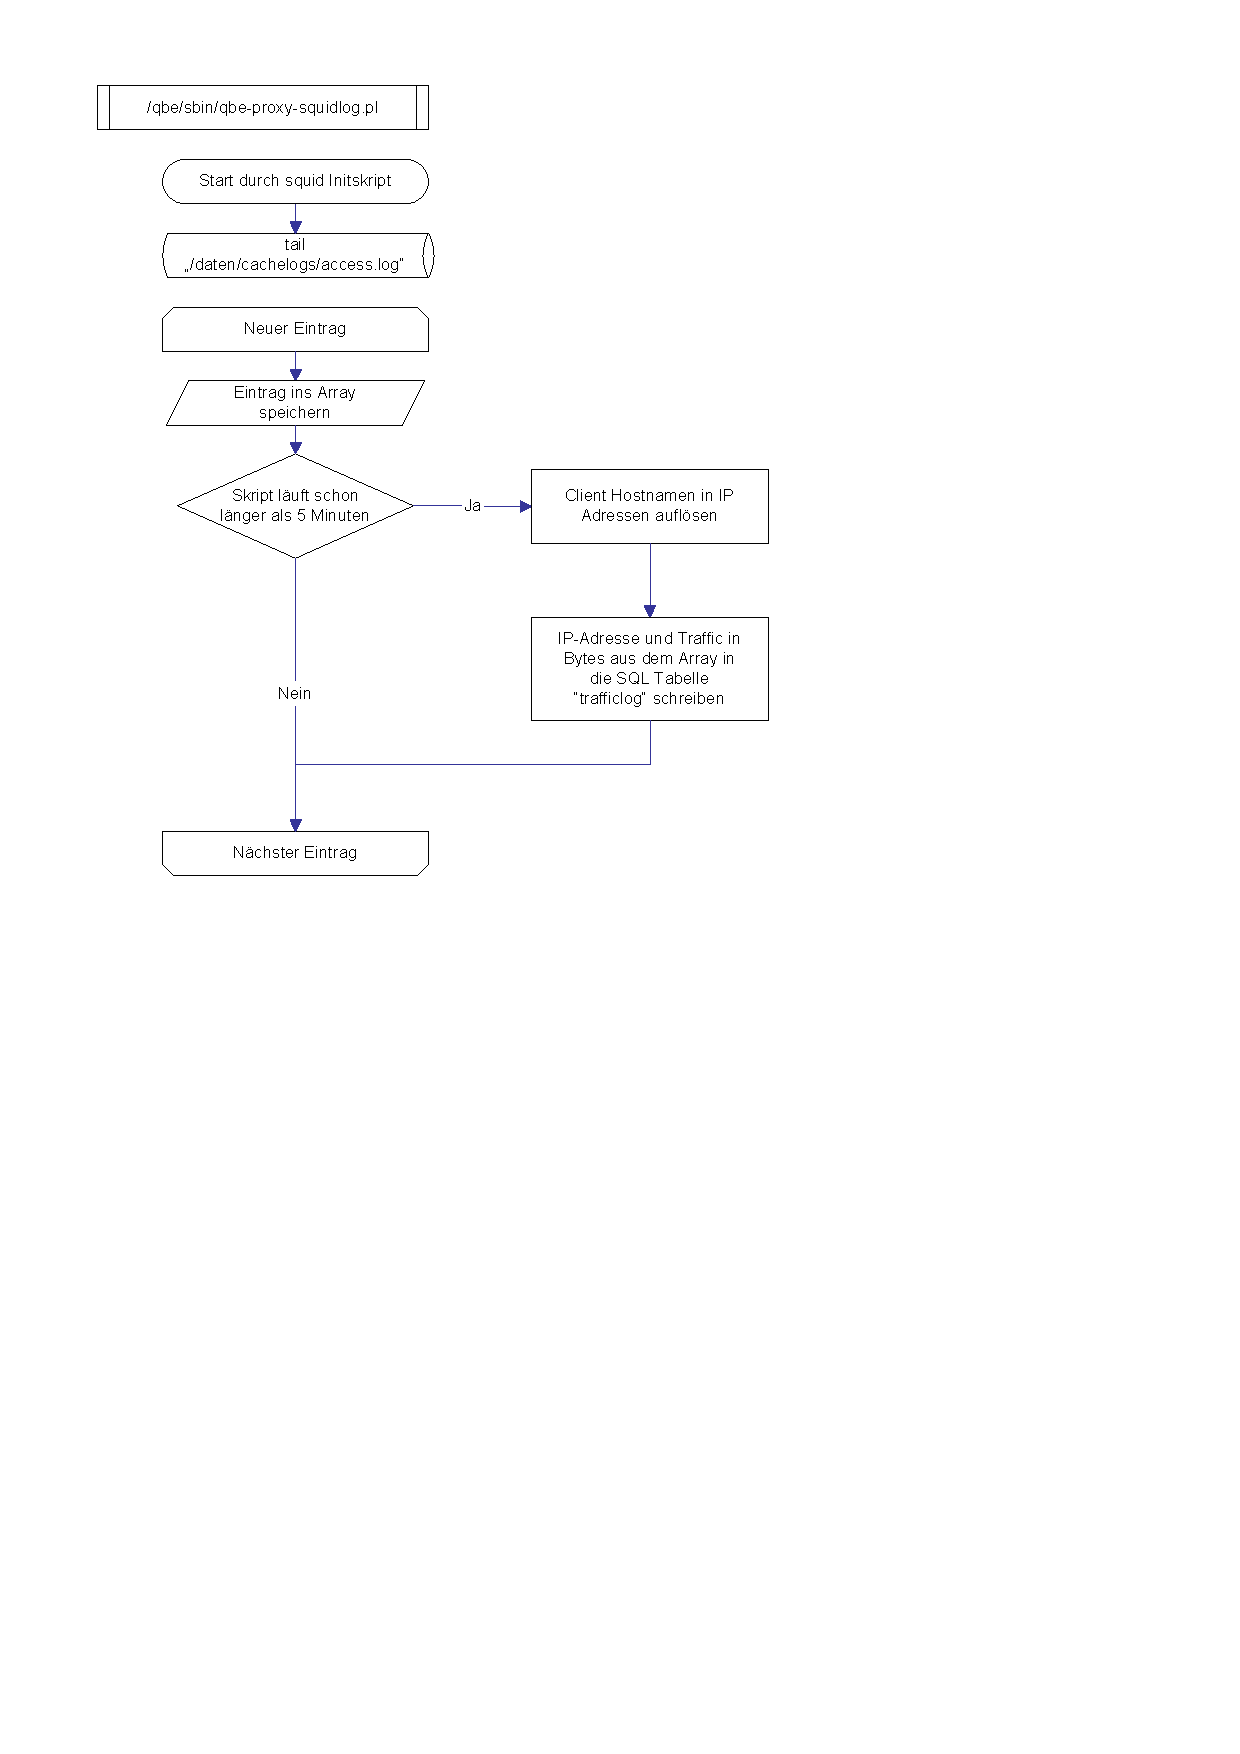
\includepdf[pagecommand={}]{files/flow-qbe-proxy-squidlog.pdf}

\subsection{Grafik-Auswertung nach Benutzern}
Am Authentication Server wird jede Stunde einmal das Skript /qbe/sbin/qbe\_trafficview.pl aufgerufen. Dieses aggregiert die Daten aus dem LDAP und kopiert die Daten pro Benutzer in die Tabelle \verb|sas.trafficview|. Die Tabelle wird im UI mittels /modules/internet/stats-traffic-overall ausgewertet und als Balkendiagramm je Abteilung dargestellt.

\begin{lstlisting}[language=sql]
CREATE TABLE trafficview (
  userid varchar(10) NOT NULL default '',
  traffic bigint(20) NOT NULL default '0',
  abt varchar(5) NOT NULL default ''
) TYPE=MyISAM;
\end{lstlisting}

Ein Beispieleintrag:
\begin{lstlisting}[language=sql]
INSERT INTO trafficview VALUES ('cb',1123132,'Adm');
\end{lstlisting}

\placefig{scr-inettraffic}{Graphische Auswertung}
\clearpage

\section{Zugriffssteuerung f�r Squid Cache}
Fr�here Qbe SAS Systeme setzten auf ein Perlskript welches regelm��ig die aktuell angemeldeten Benutzer abgefragt und in eine Datei geschrieben hat. Um die damit verbundenen Probleme zu l�sen, wird jetzt ein Modul in den Squid Cache geladen. Das Modul heisst "ip\_ldap" und wird als "external acl" eingetragen.

%Es wird eine Verbindung zum AuthServer/LDAP aufgebaut und eine Liste aller freigeschalteter Benutzer (daher Filter $(|(inetStatus=0) (inetStatus=7))$) abgerufen. Die Eintr�ge werden auf G�ltigkeit und Vorhandensein der Attribute \verb|loggedonHost| und \verb|loggedonMac| �berpr�ft. Eintr�ge, die diese Kriterien erf�llen werden im Format "\verb|loggedonHost|/32" in die Datei \verb|/qbe/data/squid.include| geschrieben.
%Um Fehlermeldungen des Squids zu vermeiden, wenn keine Benutzer angemeldet sind, wird zus�tzlich der harmlose Eintrag 127.0.0.1/32 geschrieben.

%Anschlie�end wird der \index{Squid}{Squid-Cache} angewiesen, die Konfiguration neu einzulesen. Ablaufdiagramm auf der n�chsten Seite. 
%%dazu siehe Abb. \ref{fig:flow-qbe-proxy-squidacl}

%\placefig{scr-proxyaccessdenied}{Fehlermeldung vom Proxy bei keiner Anmeldung}
%\clearpage
%%\placefig{flow-qbe-proxy-squidacl}{Ablaufdiagramm qbe-proxy-squidacl.pl}
%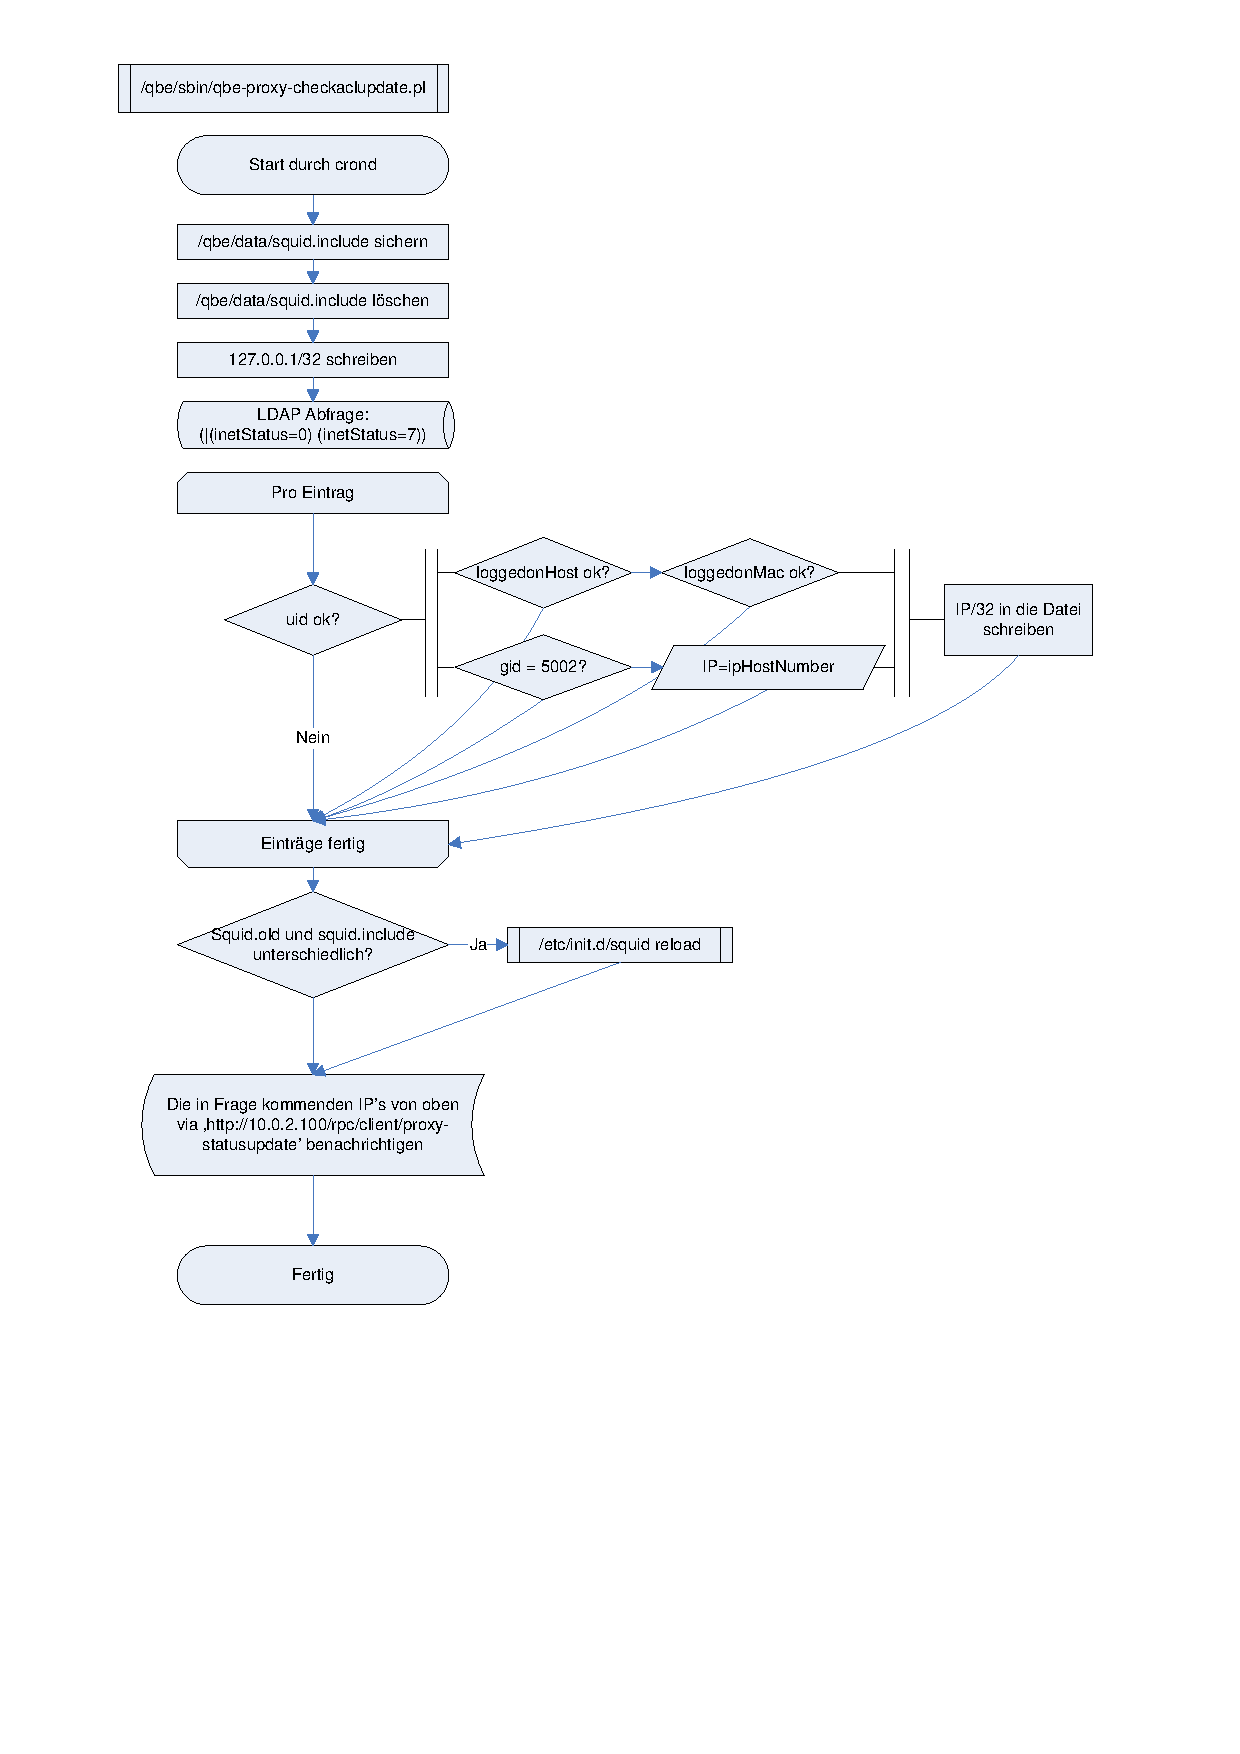
\includepdf[pagecommand={}]{files/flow-qbe-proxy-squidacl.pdf}
%

\section{�nderungen an der System-Konfiguration}

Es werden hier kurz die notwendingen �nderungen an der Standardkonfiguration eines Debian-Systems beschrieben.

\subsection{Squid: Initskript}
Das Initskript des Squid Cache daemons \verb|/etc/init.d/squid| muss angepasst werden, um \verb|qbe-proxy-squidlog.pl| entsprechend zu starten bzw. zu beenden.

Ans Ende der \verb|start()|-Routine geh�rt folgende Zeile:
\begin{lstlisting}
# Qbe SAS Proxy
/qbe/sbin/qbe-proxy-squidlog.pl&
# END
\end{lstlisting}

An den Anfang der \verb|stop()|-Routine muss folgendes hinzugef�gt werden:
\begin{lstlisting}
# Qbe SAS Proxy
killall "qbe-proxy-squidlog.pl"
# END
\end{lstlisting}

\subsection{Squid: ACL}
Um den Clients die Benutzung des Squid Caches zu erlauben, muss in der \verb|/etc/squid/squid.conf| ein \index{ACL}{ACL-Eintrag} hinzugef�gt werden:
\begin{lstlisting}
# angemeldete Benutzer
external_acl_type ldapacl ttl=45 \%SRC \%IDENT /usr/lib/squid/ip_ldap
acl proxy-users external ldapacl
\end{lstlisting}

Anschliessend mu� diese ACL in der \verb|allow|-Klasse eingetragen werden:
\begin{lstlisting}
http_access allow proxy-users
\end{lstlisting}

\section{WebSense EIM}
Soll der "WebSense Employee Internet Manager" installiert werden (der f�r �sterreichische Schulen zum Zeitpunkt des Schreibens nur einer kostenlosen Registrierung bedarf), muss mindestens Squid 2.5-STABLE verwendet werden. F�r Debian \index{Debian}{woody} ist daher ein eigenes Paket notwendig.

Mit einem kleinen Patch kann das sid-Sourcepaket (hier: 2.5.4-3) verwendet werden. Es sind dann noch zwei Pakete aus unstable zu installieren, diese sind jedoch nicht plattformabh�ngig und funktionieren ohne Modifikation.

\lstinputlisting[language=C]{files/squid-2.5.4-woody.patch}

\section{Firewall Hinweis}
Es soll hier ein Hinweis auf \verb|iptables| (bzw. \verb|ipf| oder \verb|pf| unter FreeBSD/OpenBSD) gegeben werden, mit denen eine Firewall-Funktionalit�t aufgebaut werden kann. Dies ist dringend zu empfehlen. Es sollten auch keine anderen Dienste auf dem Qbe SAS Proxy laufen (z.B. Webserver, MySQL...) da diese ein nicht einsch�tzbares Sicherheitsrisiko beherbergen k�nnen.

\section{Ideen f�r die Zukunft, bessere Skalierbarkeit}
Die in dieser Version eingesetzte ACL-Kontrolle �ber eine Datei funktioniert zwar, f�hrt jedoch teilweise zu obskuren Problemen. 
Da der Squid die ACL-Datei nur bei einem SIGHUP neu einliest, und dabei leider manchmal offene Verbindungen (warum er dies tut, ist mir unbekannt) unterbricht, w�re eine z.B. MySQL-basierende ACL besser. 
Dazu muss jedoch der Squid entsprechend erweitert werden und die Login/Logout Skripte am Authentication Server angepasst werden. 
�nderungen am Internet-Status der Benutzer k�nnte man mit einem LDAP-Event abfangen und damit die Datenbank aktualisieren.

Eine andere M�glichkeit w�re das \index{Squid}{Squid} external-acl API zu verwenden. 
Dann l�uft ein kleines Programm, dass nur mit dem \index{LDAP}{LDAP} Server spricht, sobald der squid einen Benutzer authentifizieren muss. 
Die Cache-Vorhaltezeit des Ja/Nein-Zustandes ist dann im Squid selbst konfigurierbar.

%% *eof*


% WebServer
%%
%% Qbe SAS SystemDocumentation
%% (C) Copyright 2001-2004 Christian Hofstaedtler
%%
%% $Id: part-03.tex 2 2004-03-10 08:40:26Z ch $
%%

\cChapter{Webserver Integration}
Qbe SAS ist vorbereitet um in Kooperation mit einem getrennten Webserver die Webseite der Institution und die pers�nlichen Seiten der Systembenutzer anzuzeigen.

\section{Software}
Folgende Standardsoftware wird verwendet:

\begin{Verbatim}
Debian GNU/Linux woody, RedHat Linux, alternativ FreeBSD/OpenBSD
Apache HTTP Server 1.3 oder 2.0
NFS Client
\end{Verbatim}

\section{Konfiguration}
Da keine spezielle Software verwendet wird, beschr�nkt sich die Konfiguration auf das NFS Filesystem und den Apache Webserver.

Notiz: Es ist nicht notwendig eine LDAP-Benutzerauthentifizierung einzurichten. Idealerweise gibt es auf dem Webserver nur Systemaccounts und einen Systemverwalter (nicht \verb|root|). \verb|root| sollte sich nicht remote anmelden k�nnen.

\subsection{NFS}
Datei \verb|/etc/fstab| muss um folgenden Eintrag (in einer Zeile) erg�nzt werden:

\begin{Verbatim}
10.0.2.10:/export/homes /import/homes           nfs     rw,soft,
timeo=60,async,nodev,noexec,nouser,nosuid 0 0
\end{Verbatim}

Dies wei�t das System an, beim Neustart automatisch das Filesystem mit den Benutzerverzeichnissen via NFS vom AuthServer (hier: 10.0.2.10) zu importieren. Zus�tzlich werden einige Parameter gesetzt die die Geschwindigkeit und Sicherheit positiv beeinflussen.

\subsection{Apache httpd}
In der Apache Konfigurationsdatei \verb|httpd.conf| muss folgendes sinngem�� hinzugef�gt werden (Beispiel f�r Apache 1.3):
\begin{Verbatim}
LoadModule userdir_module     modules/mod_userdir.so

<IfModule mod_userdir.c>
    UserDir disabled root
    UserDir /import/homes/*/web
</IfModule>
<Directory /import/homes/*/web>
    AllowOverride All
    Options Indexes Includes
    Order allow,deny
    Allow from all
</Directory>
\end{Verbatim}

Soll auch die Institutsseite am AuthServer abgelegt werden, kann diese im Benutzerverzeichniss des Benutzers "`web"' geschehen. Dazu muss zus�tzlich im \verb|httpd.conf| eingetragen werden:
\begin{Verbatim}
DocumentRoot "/import/homes/web"
\end{Verbatim}


%% *eof*


% Client
%%
%% Qbe SAS SystemDocumentation
%% (C) Copyright 2001-2004 Christian Hofstaedtler
%%
%% $Id: part-04.tex 20 2004-05-03 15:41:20Z ch $
%%

\cChapter{Qbe SAS Client}

\section{Systemanforderungen}

Qbe SAS Client soll prim�r auf Clientsystemen mit Betriebssystem Windows 2000 und/oder Windows XP Professional laufen. Wenn m�glich soll nur ein kleiner Teil f�r den Benutzer sichtbar sein (Anmeldung, Statusabfrage und Abmeldung) - die Funktion des Systems sollte nicht weiter in den Vordergrund ger�ckt werden. Ebenfalls soll der gesamte Clientteil nur �ber einen definierten minimalen Befehlssatz mit dem Qbe Auth Server kommunizieren und keine direkten LDAP API Aufrufe durchf�hren um maximale Portabilit�t (m�glicherweise auch von LDAP weg) zu erreichen. Bestimmte Fehler am Client sollen nicht die F�higkeit der Kommunikation mit dem Qbe Auth Server beeintr�chtigen; Netzwerk-Disconnects sollen (besonders auf Laptops) transparent behandelt werden.

\section{Betriebsarten}

Qbe SAS Client �bernimmt die Authentifizierung des Benutzers der einen beliebigen Client PC im Netzwerk benutzen m�chte. Dazu kann es in zwei verschiedenen Modi verwendet werden:

\begin{description}
\item[Network only]
Qbe SAS Client authentifiziert den Benutzer nur gegen�ber dem Server. Der Benutzer gibt seinen Benutzernamen und Passwort getrennt ein.
\item[System Logon]
Qbe SAS Client authentifiziert den Benutzer sowohl gegen�ber dem Client als auch dem Server - bereits beim anmelden an die Windows Workstation. Bei Bedarf wird ein lokaler Benutzer angelegt, und bei der Abmeldung wieder gel�scht.
\end{description}

\subsection{Serversuche}

Der zu benutzende Server wird ausschlie�lich per DNS gefunden. Standard\-m��ig benutzt Qbe SAS Client den Servernamen "qbe-auth". Die Aufl�sung des Namens in eine IP Adresse wird vom Betriebssystem durchgef�hrt - Vorraussetzungen daf�r sind:
\begin{itemize}
\item DNS-Server l�uft und ist richtig konfiguriert \\
	("qbe-auth" ist als A-Record eingetragen.)
\item Die Workstation kann den DNS-Server erreichen, und fragt mit dem richtigen Domainsuffix an. Die richtige Konfiguration der Workstation wird vorzugsweise mittels DHCP erreicht.
\end{itemize}

In der aktuell vorhandenen Version besteht keine M�glichkeit den anf�nglichen Servernamen zu �ndern. Geplant ist eine eigene DHCP-Option die vom Qbe SAS Client ausgelesen werden kann - Vorraussetzung daf�r w�re, dass die Workstation die IP-Stack Konfiguration vom DHCP-Server bekommt.

\begin{Verbatim}
; DNS-Beispieleintrag:
qbe-auth.htlwrn.ac.at.	IN	A		10.0.2.100
\end{Verbatim}

 
\subsection{Einzelteile}

Der Qbe SAS Client ist ein komplexes System, dass aus vielen kleineren Teilen besteht:

\begin{tabular}{|l|l|l|}
\hline
Teilsystem & Dateiname \\
\hline
Network Authentication Service & QbeSvc.exe \\
 & QbeSAS.dll \\
System Logon & QbeGina.dll \\
Statusanzeige & QbeTray.exe  \\
UI Components & iLogin.hta \\
& startup.hta \\
& Q.ico \\
COM API	& iLoginCOM.dll	\\
Einstellungen & iLogin.reg \\
Installation & ServicePack.exe \\
 & netQbe.inf \\
 & QbeNDI.exe \\
\hline
\end{tabular}

Qbe SAS Client kann bereits mit nur dem installiertem "qbesvc.exe" im "Network only" Modus betrieben werden - f�r den "System Logon" Modus bzw. f�r eine benutzerfreundliche Umgebung sollte der Client vollst�ndig installiert werden.


%\begin{center}
%	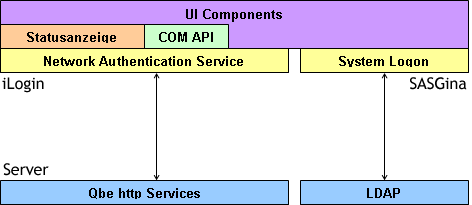
\includegraphics[width=1.00\textwidth]{files/pic-03-beziehungsdiagramm}
%\end{center}
\placefig{pic-03-beziehungsdiagramm}{Beziehungsdiagramm Qbe SAS Client/Server}


Im Beziehungsdiagramm wird deutlich, dass der Network Authentication Service alle grundlegenden Dienste f�r den iLogin Client zur Verf�gung stellt. Wird der System Logon Mode benutzt, wird ein zus�tzlicher Teil systemwichtig -- die SASGina. Dieser wird in das Windows Login eingebunden, und �bernimmt die Windows Anmeldung, LDAP Benutzer�berpr�fung und Datenspeicherung.

\subsubsection{Network Authentication Service}

Dieser l�uft als Windows-Dienst und implementiert sowohl einen HTTP-SSL Client f�r die Kommunikation mit dem Qbe-Auth Server, als auch einen HTTP Server (auf TCP/IP Port 7666) der die Interaktion mit dem Benutzer erm�glicht und Teile des Authentifizierungshandshakes abarbeitet. Auf den Network Authentication Service kann mit einem normalen Webbrowser zugegriffen werden, speziell wurde dies aber f�r den Internet Explorer (bzw. f�r die Microsoft HTML Engine) entwickelt und optimiert, da die restlichen Benutzerinterface-Teile auf der Microsoft HTML Engine aufsetzen. 

Alle weiteren Teile kommunizieren ausschlie�lich mit dem Network Authentication Service der alle relevanten Daten �ber den Benutzer im Speicher h�lt - diese Daten werden regelm��ig vom Server aufgefrischt.

Der HTTP Server erm�glicht es dem Server au�erdem, bestimmte Parameter (Benutzername, Servername, Letzte Verbindung, ...) abzufragen sowie Programme auszuf�hren (etwa um einen Drucker zu installieren). Dies wird durch eine Abfrage der IP-Adresse gesch�tzt.

\subsubsection{COM API and Authentication Helper}

Das COM API erm�glicht es auf den Network Authentication Service per Microsoft COM (ActiveX) zuzugreifen. Gleichzeitig erlaubt es eine Speicherung der Benutzerdaten (Username und Passwort) in der Registry um die Anmeldung zu beschleunigen. Wird iLogin im System Logon oder Single Sign On Mode betrieben, holt das COM API den Benutzernamen und Passwort vom Windows System. \\


\subsubsection{Statusanzeige}

Die Statusanzeige besteht aus einem Windows System Tray Symbol dass den aktuellen Internetstatus signalisiert, wichtige Ereignisse dem Benutzer mitteilt und schnellen Zugriff auf die iLogin Statusseite und Anmeldung erlaubt.
F�r die Statusseite und Anmeldung werden die "UI Components" gestartet.
Energie-Events werden vom iLogin Tray Symbol behandelt. Bei einem kritischen Energieereignis (Standby/Ruhezustand) wird versucht eine Abmeldung durch den Network Authentication Service zu erreichen. 30 Sekunden nach dem Aufwachen wird eine transparente Verbindungswiederherstellung eingeleitet.

\subsubsection{UI Components}

Die sogenannten UI Components bestehen lediglich aus Beschreibungsdateien f�r \href{http://msdn.microsoft.com/workshop/author/hta/overview/htaoverview.asp}{Microsoft HTA Applikationen}, die auf den http Server im Network Authentication Service verweisen.

\placefig{scr-win32client}{Screenshot Qbe SAS Client unter Windows}

\subsubsection{Einstellungen}

Qbe SAS Client installiert bei der Anmeldung einige Standardeinstellungen (z.B. Proxykonfiguration), die direkt aus der Datei "iLogin.reg" kommen. Diese wird mit Hilfe vom Windows Registrierungseditors automatisch in die Registry importiert.

\subsubsection{Update}
Da der Client bei jeder Anmeldung die Versionsnummer an den Server sendet, k�nnen alte/problematische Client-Versionen einfach ausgeschlossen werden. Clients die den Statuscode \verb|404 - Not found| erhalten, sollten keine weitere Anfrage an den Server schicken.

Neuere Windows Clients (ab 2.01) stellen die Benutzerschnittstelle erst nach einer Anfrage an den Server dar. Damit kann ein Update des Clients erzwungen werden. Workstations mit HDGUARD werden am Client abgefragt und das Zwangupdate wird �bersprungen.


\section{Installation}
\subsection{Qbe SAS Client}
Das Setup bietet keine Optionen an und installiert alle Dateien nach \%SystemRoot\%/System32/Qbe/Setup. Die Reihenfolge:
\begin{itemize}
\item[-] .NET VM wird gegebenenfalls heruntergeladen und installiert.
\item[-] \%SystemRoot\%/System32/Qbe/Setup wird komplett gel�scht.
\item[-] PFC wird in das System kopiert und ausgef�hrt (siehe unten)
\item[-] Dateien von fr�heren Versionen die nach \%SystemRoot\%/System32 und \%ProgramFiles\%/iLogin installiert wurden werden gel�scht
\item[-] Alle Dateien werden nach \%SystemRoot\%/System32/Qbe/Setup kopiert
\item[-] Windows NDI installiert den Qbe SAS Client als NetService-Komponente
\item[-] QbeGina wird nicht automatisch installiert/upgedated
\end{itemize}

\subsection{PFC}
Qbe "Pre-Flight-Check" ist eine .NET Anwendung (ClientSource/SetupPFC) die vor der eigentlichen Installation ausgef�hrt wird und folgende Tasks erledigt:
\begin{itemize}
\item vorherigen Versionen von QbeSvc, QbeTray, iLogin, etc. schliessen
\item QbeSvc aus der Registry entfernen
\item HTA-Ausf�hrungsschicht (MSHTA) beenden
\item Windows Service-Pack �berpr�fen und ggf. das aktuelle Service Pack installieren
\end{itemize}

\subsection{Wizard}
Es ist ein Installationswizard geplant der den Benutzer durch die Schritte Client Installation, Computerkonfiguration, Account Aktivierung und Netzwerkkarte registrieren f�hrt. Dieser wurde bereits in .NET angefangen, ist jedoch nicht fertig. (Projektverzeichnis ClientSource/Wizard)

\subsection{System-Updates}

Der SAS Client (f�r Windows) ben�tigt Windows 2000 oder XP mit installiertem .NET Framework. Das aktuelle Servicepack auf den Zielsystemen ist nicht zwingend erforderlich, w�re aber von Vorteil.
Das Client Setup pr�ft vor der eigentlichen Client-Installation ob das .NET Framework und die Microsoft C++ 7.1 Runtimes vorhanden ist - wenn nicht wird beides heruntergeladen und installiert.

\subsubsection{.NET Framework}
F�r das .NET Framework wird mittels Registry-Key die Installation �berpr�ft, andernfalls wird das Setup heruntergeladen und gestartet. Kein Setup-Neustart.

\begin{Verbatim}
URL: http://qbe-auth.htlwrn.ac.at/login/dotnetfx.exe

ch@xtc:/qbe/web/htdocs/login -> ls -la dotnetfx.exe
-rw-rw-r--  ch   sysops   24277024 Mar  4  2003 dotnetfx.exe
\end{Verbatim}	

\subsubsection{Service-Pack}
F�r das Service-Pack wird die NSI-Anwendung (ClientSource/Setup/ServicePack.nsi) gestartet die dann vom AuthServer das ServicePack herunterl�dt und installiert.
Die ServicePack Installationsdateien dazu liegen am AuthServer im /login/ Verzeichniss.
\begin{Verbatim}
URL: http://qbe-auth.htlwrn.ac.at/login/servicepack.php?ver=5.0

ch@xtc:/qbe/web/htdocs/login -> ls -la service*exe
-rwxrw-r--  ch   sysops   135945992 Jun 20  2003 servicepack-5.0.exe
-rwxrw-r--  ch   sysops   129049184 Jan 27  2003 servicepack-5.1.exe
\end{Verbatim}

\subsection{Client kompilieren}
Es werden kurz die Vorraussetzungen und der Kompilationsvorgang selbst beschrieben.

\subsubsection{Vorraussetzungen}
Um die Qbe SAS Client Sourcen zu kompilieren muss folgende Software auf dem Entwicklungssystem gegeben sein:

\begin{itemize}
\item Microsoft Visual Studio 6.0
\item Microsoft Visual Studio .NET 2003
\item Microsoft Windows XP SP1 DDK
\item Microsoft Platform SDK (February 2003)
\item GCC 3.x aus dem Cygwin Paket
\item Nullsoft Install System 2.0
\end{itemize}

Es muss die Umgebungsvariable \verb|%DEVELDRIVE%| gesetzt sein. Zum Beispiel: \verb|set DEVELDRIVE=C:| wenn die Software auf C: installiert wurde.
Weiters darf keines der Visual Studio Setups den PATH oder LIBS/INCLUDE etc. ver�ndert haben. Diese Variablen werden durch das build-Skript automatisch f�r das Microsoft Platform SDK gesetzt.

\subsubsection{NSIS Patch}
Der SAS Client Installer erfordert folgenden Patch des "NSISdl" Modules.

\VerbatimInput{files/nsisdl-noproxy.patch}

\subsubsection{Kompilierungsskript}
Um die Erstellung des Qbe SAS Client Installers drastisch zu vereinfachen wurden alle Komponenten -- Die .NET Komponenten m�ssen zuerst h�ndisch kompiliert werden. -- mit einem Makefile versehen. Die Makefiles werden durch das Skript "buildx.bat" aufgerufen, welches wiederum �ber eines der build-w2k.bat oder build-wxp.bat aufgerufen wird. Die build-xxx.bat Skripte starten zuerst das Platform SDK setenv.bat mit Parametern um das Build-Environment entsprechend herzurichten. Anschliessend wird buildx.bat ausgef�hrt... Die Zieldateien werden im Verzeichnis BIN/RETAIL/PLATFORMNAME erstellt. 

\subsubsection{Versionsnummern}
Die Versionsnummer wird in der Datei C/ilogin-version.h definiert. Die Datei wird von sehr vielen Komponenten benutzt um die Qbe SAS Client Ziel-Version zu ermitteln und darzustellen.

\section{Qbe SAS Xplat Client}

Der komplexe Aufbau und die enge Verwebung mit dem Windows Betriebssystem machen es (mit heutigen Mitteln) unm�glich den normalen Qbe SAS Client unter z.B. Linux zu verwenden. 

Auf der anderen Seite macht die .NET Architektur dies sehr einfach. So kann, mit der Annahme dass es pro PC nur einen Benutzer gibt, der gleiche Sourcecode verwendet werden, um ein mit Mono ausf�hrbares Binary zu erstellen.
Dieses Binary ("QbeService.exe") enth�lt dann die minimalste Funktionalit�t, die der Qbe SAS Client mitbringen muss. Da das User Interface hier ebenfalls �ber HTTP ausgeliefert wird, sieht der Client f�r den Endanwender relativ �hnlich zum Windows Client aus.

\placefig{scr-unixclientui}{Screenshot: Qbe SAS Client unter Linux: Benutzeroberfl�che}

Zus�tzlich zu dem QbeService.exe sind im Source-Tree ein paar Skripte die die Verwendung mit Gnome als X11-Umgebung erleichtern k�nnen.

\placefig{scr-unixclientshell}{Screenshot: Qbe SAS Client unter Linux: Terminalfenster}

\section{System Logon}
Die QbeGina und unterst�tzende Dateien werden mit dem "Windows Logon Enabler" Setup installiert.
Die aktuelle Version implementiert eine transparente LDAP-Authentifizierung. Benutzer werden automatisch angelegt bzw. gel�scht. Homedirectory wird entsprechend eingestellt, der Profilpfad wird auf \%HOMEDRIVE\%/profile gesetzt. Im Anmeldedialogfeld kann mit der Tastenkombination CTRL-ALT-DEL die LDAP-Authentifizierung �bersprungen werden -- dann wird die normale MSGina.dll f�r diese Session aktiv.

Das Setup �ndert folgende Einstellungen:

\begin{itemize}
\item Der Registry-Key HKLM/Software/Microsoft/Windows NT/CurrentVersion/Winlogon/GinaDLL wird auf "QbeGina.dll" gesetzt.
\item HKLM/SOFTWARE/Microsoft/Windows NT/CurrentVersion/Winlogon wird auf den Computer Namen gesetzt.
\item Die Gruppe "Qbe SAS Users" wird angelegt.
\item Unter HKLM/SYSTEM/CurrentControlSet/Services wird ein neuer Netzwerk-Provider "QbeNP" angelegt.
\item QbeNP wird in HKLM/SYSTEM/CurrentControlSet/Control/NetworkProvider/Order/ProviderOrder hinzugef�gt.
\end{itemize}

Die Arbeitsweise der Systemanmeldung wird in den Abbildungen \ref{fig:qbegina-workflow-p1} bis \ref{fig:qbegina-workflow-p3} ersichtlich.

\begin{flushleft}
\placefigx{qbegina-workflow-p1}{Ablaufdiagramm: QbeGina Initialisierungsvorgang}{width=6cm}
\placefigx{qbegina-workflow-p2}{Ablaufdiagramm: QbeGina Benutzeranmeldung}{width=6cm}
\placefigx{qbegina-workflow-p3}{Ablaufdiagramm: QbeGina Benutzerabmeldung}{width=6cm}
\placefigx{scr-qbegina-ctrlaltdel}{Screenshot: QbeGina Fenster vor der Anmeldung}{width=6cm}
\placefigx{scr-qbegina-ldapconnlost}{Screenshot: QbeGina Anmeldung wenn die LDAP Verbindung verloren geht}{width=6cm}
\placefigx{scr-qbegina-loginwithuser}{Screenshot: QbeGina Benutzeranmeldefenster}{width=6cm}
\newpage
\end{flushleft}

\section{Client/Server-Protokollbeschreibung}

Der Qbe SAS Client und der Qbe Authentication Server benutzen eine eigene, einfache RPC-over-HTTP Implementation.

\subsection{UserAgent Feldbeschreibung}
Der Qbe SAS Client soll/muss immer einen UserAgent-Header mitschicken, der den Client als Client mit definierter Versionsnummer identifiziert. Der Feldaufbau f�r alte Versionen ist wie folgend:
\begin{itemize}
\item Zeichenkette "iLogin"
\item Leerzeichen
\item Der Programmname. Zum Beispiel "QbeService (WIN32)"
\item Leerzeichen
\item Qbe SAS Client Versionsnummer. Zum Beispiel "2.23.00"
\end{itemize}

Beginnend mit 2.23.10, wird folgendes Format verwendet:

\begin{itemize}
\item Zeichenkette "QbeService/"
\item Qbe SAS Client Versionsnummer. Zum Beispiel "2.23.89"
\end{itemize}

Der Server muss sich dem Client gegen�ber nicht ausweisen. Die neuen Clients melden den Platform-Namen nicht mehr an den Server.

\subsection{Server-Befehle}
Folgende Befehle sind am Server zur Benutzung durch den Client implementiert:

\subsubsection{/rpc/client/login}
Meldet einen Benutzer am System an. Der Anmeldevorgang besteht aus der Benutzername/Passwort-�berpr�fung am LDAP Server und der Eintragung der aktuellen IP- und MAC-Adresse des Clients.

Akzeptiert die GET-Parameter "user" und "pass" f�r Testzwecke, oder vom Client die Header "iLogin-User" (Benutzername), "iLogin-Pass" (Passwort), "iLogin-Token" (Benutzername/Passwort base64 enkodiert). Auf jeden Fall muss der GET-Paramter "ver" (die Client-Versionsnummer) vorhanden sein.

Die Antwort besteht aus dem HTTP Statuscode, sowie dem Internet-Status aus dem LDAP ("iLogin-User-State"), dem bisherigen Internettraffic ("iLogin-Stats-Traffic") und der Speicherplatznutzung ("iLogin-Stats-Disk"). 

Der HTTP Statuscode kann folgende Werte annehmen:
\begin{itemize}
\item 200 OK, Anmeldung erfolgreich
\item 401 Fehler: Benutzer muss zuerst Passwort �ndern
\item 403 Fehler: Benutzername/Passwort falsch
\item 404 Fehler: Das API hat sich ge�ndert, bzw. der Qbe SAS Client ist veraltet.
\item 500 Fehler: Allgemeiner Serverfehler. Client soll die Anmeldung nicht erneut versuchen.
\end{itemize}

\subsubsection{/rpc/client/logout}
Meldet den aktuellen Benutzer vom System ab. Akzeptiert keine Parameter und liefert immer HTTP-Statuscode 200 ("OK") zur�ck.

\subsubsection{/rpc/client/svc-top.php}
Zeigt die Zeichenfolge "Qbe SAS Client [Versionsnummer]", wobei die [Versionsnummer] aus dem GET-Parameter "ver" verwendet wird. Wird der "ver"-Parameter nicht angegeben, wird als [Versionsnummer] der String "�" benutzt.

Ab Qbe Application Server 0.91 wird zus�tzlich auch ein Hinweis auf den Serverstatus angezeigt. "ok" bzw. "fail".

\subsubsection{/rpc/client/svc-frame.php}
Erstellt ein HTML Frameset zur Verwendung in der Windows-Version des Qbe SAS Clients. Enth�lt ein Top-Frame mit dem "svc-top.php" und ein Content-Frame mit entweder der QbeSvc-URL "http://127.0.0.1:7666/web/menu" oder der Update-Info "update.php"

\subsubsection{/rpc/client/update.php}
Wei�t auf eine neue verf�gbare Qbe SAS Client Version hin. Auf PCs mit installiertem HDGUARD wird der Hinweis mittels einem VBScript/Registry-Check �bersprungen.

\subsection{Client-Befehle}

Die Client-Befehle sind unter Windows im QbeSvc.EXE, im Xplat Client im QbeService.EXE implementiert. Befehle werden nur von IPs im Bereich 10.0.2.0/24 akzeptiert.
Befehle mit Pr�fix "/web" sollten nicht vom Server sondern nur intern vom Qbe SAS Client benutzt werden.

\subsubsection{/}
Optional: Weiterleitung nach "/web/menu".

\subsubsection{/web/menu}
Optional: Zeigt eine einfache �bersicht �ber den Status des Qbe SAS Client zur lokalen Verwendung an. �blicherweise werden der Benutzername, der Servername, Zeit der letzten Verbindung, eventuell der letzte Fehler bzw. die Benutzerstatistiken angezeigt.

\subsubsection{/web/login}
Optional: Zeigt das Anmeldeformular zur lokalen Verwendung an. Mittels ActiveX Objekt wird ein eventuell vorher gespeichertes Benutzername/Passwort-Paar aus der Registry ausgelesen und abgeschickt. Andernfalls kann man das Paar abspeichern.

Das Formular f�hrt einen POST-Request auf "/auth/setlogin" aus.

\subsubsection{/web/hta-login}
Optional: Hilfsdaten f�r den Windows Client.

\subsubsection{/web/hta-login-done}
Optional: Hilfsdaten f�r den Windows Client.

\subsubsection{/web/hta-login-post}
Optional: Hilfsdaten f�r den Windows Client.

\subsubsection{/web/cleardata}
Optional: L�scht ein eventuell vorher gespeichertes Benutzername/Passwort-Paar via ActiveX-Objekt aus der Registry.

\subsubsection{/web/logout}
Optional: Initiert eine Abmeldung im Hintergrund.

\subsubsection{/auth/login}
Initiiert eine Hintergrundanmeldung.

\subsubsection{/auth/setauthserver}
Optional: Akzeptiert im GET-Parameter "server" einen neuen Namen f�r den Qbe Authentication Server. Default: "qbe-auth"

\subsubsection{/auth/setlogin}
Akzeptiert die GET-Daten des Formulars "/web/login" und initiiert eine Hintergrundanmeldung.

\subsubsection{/auth/logout}
Initiert eine Abmeldung im Hintergrund.

\subsubsection{/auth/forcerefresh}

\subsubsection{/service/stop}
Optional: Windows-Spezifisch: Beendet den QbeSvc.

\subsubsection{/system/exec}
Optional: Windows-Spezifisch: F�hrt einen Befehl im Kontext des QbeSvc aus.

\subsubsection{/system/setmanager}
�bernimmt den GET-QueryString als neue zus�tzliche Manager-IP von der Befehle entgegen genommen werden.

\subsubsection{/system/getinfo}
Akzeptiert den GET-Parameter "type" und liefert die gew�nschte Information zur�ck. G�ltige Werte sind:

\begin{itemize}
\item osversion Optional: Die Betriebssystemversion.
\item osregowner Optional: Der Name des Benutzers auf den das Betriebssystem eingetragen wurde.
\item hostname Der Computername.
\item username Der Qbe SAS Benutzername oder "*VOID*" wenn kein Benutzername bekannt ist.
\item authtoken Das Qbe SAS Benutzername/Passwort-Token oder "*VOID*" wenn kein Benutzername/Passwort-Token bekannt ist.
\item version Die Qbe SAS Clientversion.
\item cvsid Optional: Die CVS bzw. SVN \$Id\$.
\item copyright Optional: Die Copyright-Information des installierten Qbe SAS Client.
\item time Optional: Die aktuelle Zeit.
\item authserver Der verwendete Qbe Authentication Server
\item connectionstate Optional: Der zuletzt bekannte Zustand der Systemverbindung.
\item internetstate Optional: Der zuletzt bekannte Internet-Zustand des Benutzers.
\end{itemize}

\subsubsection{/system/message}
Sendet den GET-QueryString als Nachricht an den Benutzer.

\subsubsection{/system/shutdown}
Optional: F�hrt den Computer herunter.

\subsubsection{/system/restart}
Optional: Startet den Computer neu.

\subsubsection{/ilogin/update}
Server best�tigt eine Anmeldung oder sendet einen Keep-Alive-Request. Gleichzeitig werden der Internetstatus, die Internetnutzung in Prozent und die Speicherplatznutzung in Prozent �bertragen.

\subsubsection{/ilogin/logout}
Server best�tigt eine Abmeldung. Client l�scht alle relevanten Daten.

\subsubsection{/ilogin/time}
Optional: Server sendet die aktuelle Zeit in Sekunden seit 1. 1. 1970 an den Client. Dieser sollte dann die Systemzeit richtig einstellen.

\subsection{Ablaufdiagramme}

FIXME: Ablauf Login, Refresh

%% *eof*


% Protocol
%%
%% Qbe SAS SystemDocumentation
%% (C) Copyright 2001-2004 Christian Hofstaedtler
%%
%% $Id: part-04.tex 24 2004-05-07 06:28:49Z ch $
%%

\cChapter{Client/Server Protokoll}
\label{chap-csprotocol}

Der Qbe SAS Client und der Qbe Authentication Server benutzen eine eigene, einfache \index{RPC}{RPC} Implementation, die auf HTTP aufsetzt. Verbindungen vom Server zum Client sind immer unverschl�sselt, in die andere Richtung steht es dem Client frei zwischen \index{HTTP}{HTTP} und \index{HTTP-SSL}{HTTP-SSL} zu w�hlen.

\section{UserAgent Feldbeschreibung}
Der Qbe SAS Client sollte immer einen UserAgent-\index{Header}{Header} mitschicken, der den Client als richtigen Client mit definierter Versionsnummer identifiziert. Der Feldaufbau f�r alte Versionen ist wie folgend:
\begin{itemize}
\item Zeichenkette "iLogin"
\item Leerzeichen
\item Der Programmname. Zum Beispiel "QbeService (WIN32)"
\item Leerzeichen
\item Qbe SAS Client Versionsnummer. Zum Beispiel "2.23.00"
\end{itemize}

Beginnend mit Client Version 2.23.10 wird folgendes Format verwendet:
\index{QbeService}

\begin{itemize}
\item Zeichenkette "QbeService/"
\item Qbe SAS Client Versionsnummer. Zum Beispiel "2.23.89"
\end{itemize}

Clients, die nicht diesen Anforderungen entsprechen, werden eventuell vom Server abgewiesen. 
Die neuen Clients melden den Betriebssystemnamen nicht mehr an den Server.

\section{Server API}
Folgende Befehle sind am Server zur Benutzung durch den Client implementiert:

\subsection{/rpc/client/login}
�berpr�ft den Benutzernamen und das Passwort gegen�ber dem \index{LDAP}{LDAP} Verzeichnis und tr�gt dann die aktuelle IP- und MAC-Adresse des Clients in das Benutzerobjekt ein. Ist bereits eine IP- oder MAC-Adresse eingetragen, werden diese �berschrieben und alte Anmeldungen werden damit ung�ltig.

Akzeptiert die GET-Parameter "user" und "pass" f�r Testzwecke, oder vom Client die \index{Header}{Header} "iLogin-User" (Benutzername), "iLogin-Pass" (Passwort), oder "iLogin-Token" (Benutzername/Passwort base64 enkodiert). Auf jeden Fall muss der GET-Paramter "ver" (die Client-Versionsnummer) und der "UserAgent"-Header vorhanden sein.

Die Antwort besteht aus dem \index{HTTP}{HTTP} Statuscode, sowie dem Internet-Status aus dem LDAP ("iLogin-User-State"), dem bisherigen Internettraffic ("iLogin-Stats-Traffic") und der Speicherplatznutzung ("iLogin-Stats-Disk"). 

Der HTTP \index{Statuscode}{Statuscode} kann folgende Werte annehmen:
\begin{itemize}
\item 200 OK, Anmeldung erfolgreich
\item 401 Fehler: Benutzer muss zuerst Passwort �ndern
\item 403 Fehler: Benutzername/Passwort falsch
\item 404 Fehler: Das API hat sich ge�ndert, bzw. der Qbe SAS Client ist veraltet.
\item 500 Fehler: Allgemeiner Serverfehler. Client soll die Anmeldung nicht erneut versuchen.
\end{itemize}

Die Anmeldeversuche und Resultate werden mittels \index{syslog}{syslog} nach /var/log/qbe.log gespeichert.

\subsection{/rpc/client/logout}
Meldet den aktuellen Benutzer vom System ab. Akzeptiert keine Parameter und liefert immer HTTP-Statuscode 200 ("OK") zur�ck.

Zur Abmeldung wird nach dem ersten LDAP-Eintrag, der auf den folgender Filter passt gesucht: \textit{(loggenonHost=\$ClientIP)}. In diesem Eintrag werden dann die Attribute loggedon\-Host, loggedon\-Mac, und last\-Activity gel�scht.

Die Abmeldungen werden mittels \index{syslog}{syslog} nach /var/log/qbe.log gespeichert.

\subsection{/rpc/client/svc-top.php}
Zeigt den Schriftzug "Qbe SAS Client MJ.MN.RV" (wobei MJ = Majorversion, MN = Minorversion, RV = Revision des Clients) auf blauem Hintergrund. 

Ab Qbe Application Server Version 0.91 wird zus�tzlich auch ein Hinweis auf den Serverstatus angezeigt. z.B: Server: ok. Andere Zust�nde k�nnen fail oder critical sein.

\subsection{/rpc/client/svc-frame.php}
Erstellt ein HTML Frameset zur Verwendung in der Windows-Version des Qbe SAS Clients. Enth�lt ein Top-Frame mit dem \verb|svc-top.php| und ein Content-Frame mit der QbeSvc-URL "http://127.0.0.1:7666/web/menu".
Wird vom Client im Parameter \verb|ver| eine Versionsnummer �bermittelt und entspricht diese nicht der aktuellen Version, wird statt dem Content Frame die Update-Info Seite \verb|update.php| angezeigt.

\subsection{/rpc/client/update.php}
Weist auf eine neue verf�gbare Qbe SAS Client Version hin. Auf PCs mit installiertem \index{HDGuard}{HDGuard} wird der Hinweis mittels einem VBScript/Registry-Check �bersprungen.

\section{Client API}

Die Client-Befehle sind unter Windows im QbeSvc.EXE, im Xplat Client im QbeService.EXE implementiert. Befehle werden nur von IPs im Bereich 10.0.2.0/24 akzeptiert, der Server muss sich jedoch nicht weiter ausweisen.

Befehle mit Pr�fix "/web" sollten nicht vom Server, sondern nur intern vom Qbe SAS Client benutzt werden.

Der Client antwortet im Fehlerfall mit \index{Statuscode}{Statuscode} 400 oder 404. Code 400 wird f�r nicht implementierte Methoden (HEAD, POST) verwendet, 404 f�r nicht implementierte Pfade.

\subsection{/}
Optional: Weiterleitung nach "/web/menu".

\subsection{/web/menu}
Optional: Zeigt eine einfache �bersicht �ber den Status des Qbe SAS Client zur lokalen Verwendung an. �blicherweise werden der Benutzername, der Servername, Zeit der letzten Verbindung, eventuell der letzte Fehler bzw. die Benutzerstatistiken angezeigt.

\subsection{/web/login}
Optional: Zeigt das Anmeldeformular zur lokalen Verwendung an. Mittels ActiveX Objekt wird ein eventuell vorher gespeichertes Benutzername/Passwort-Paar aus der Registry ausgelesen und abgeschickt. Andernfalls kann man das Paar abspeichern.

Das Formular f�hrt einen GET-Request auf "/auth/setlogin" aus.

\subsection{/web/hta-login}
Optional: Hilfsdaten f�r den Windows Client.

\subsection{/web/hta-login-done}
Optional: Hilfsdaten f�r den Windows Client.

\subsection{/web/hta-login-post}
Optional: Hilfsdaten f�r den Windows Client.

\subsection{/web/cleardata}
Optional: L�scht ein eventuell vorher gespeichertes Benutzername/Passwort-Paar via ActiveX-Objekt aus der Registry.

\subsection{/web/logout}
Optional: Initiiert eine Abmeldung im Hintergrund.

\subsection{/auth/login}
Initiiert eine Hintergrundanmeldung.

\subsection{/auth/setauthserver}
Optional: Akzeptiert im GET-Parameter "server" einen neuen Namen f�r den Qbe Authentication Server. Default: "\index{qbe-auth}{qbe-auth}"

\subsection{/auth/setlogin}
Akzeptiert die GET-Daten des Formulars "/web/login" und initiiert eine Hintergrundanmeldung.

\subsection{/auth/logout}
Initiiert eine Abmeldung im Hintergrund.

\subsection{/auth/forcerefresh}

\subsection{/service/stop}
Optional: Windows-Spezifisch: Beendet den QbeSvc.

\subsection{/system/exec}
Optional: Windows-Spezifisch: F�hrt einen Befehl im Kontext des QbeSvc aus.

\subsection{/system/setmanager}
�bernimmt den GET-QueryString als neue zus�tzliche Manager-IP, von der Befehle entgegen genommen werden.

\subsection{/system/getinfo}
Akzeptiert den GET-Parameter "type" und liefert die gew�nschte Information zur�ck. G�ltige Werte sind:

\begin{description}
\item[osversion] Optional: Die Betriebssystemversion.
\item[osregowner] Optional: Der Name des Benutzers auf den das Betriebssystem eingetragen wurde.
\item[hostname] Der Computername.
\item[username] Der Qbe SAS Benutzername oder "*VOID*" wenn kein Benutzername bekannt ist.
\item[authtoken] Das Qbe SAS Benutzername/Passwort-Token oder "*VOID*" wenn kein Benutzername/Passwort-Token bekannt ist.
\item[version] Die Qbe SAS Clientversion.
\item[cvsid] Optional: Die CVS bzw. SVN \$Id\$.
\item[copyright] Optional: Die Copyright-Information des installierten Qbe SAS Client.
\item[time] Optional: Die aktuelle Zeit.
\item[authserver] Der verwendete Qbe Authentication Server
\item[connectionstate] Optional: Der zuletzt bekannte Zustand der Systemverbindung.
\item[internetstate] Optional: Der zuletzt bekannte Internet-Zustand des Benutzers.
\end{description}

\subsection{/system/message}
Sendet den GET-QueryString als Nachricht an den Benutzer.

\subsection{/system/shutdown}
Optional: F�hrt den Computer herunter.

\subsection{/system/restart}
Optional: Startet den Computer neu.

\subsection{/ilogin/update}
Server best�tigt eine Anmeldung oder sendet einen Keep-Alive-Request. Gleichzeitig werden der Internetstatus, die Internetnutzung in Prozent und die Speicherplatznutzung in Prozent �bertragen.

\subsection{/ilogin/logout}
Server best�tigt eine Abmeldung. Client l�scht alle relevanten Daten wie Benutzername, Passwort, letzte Kommunikationszeit, Internetstatus \ldots

\subsection{/ilogin/time}
Optional: Server sendet die aktuelle Zeit in Sekunden seit 1. 1. 1970 an den Client. Dieser sollte dann die Systemzeit richtig einstellen.

\placefigx{flow-client-login}{Ablaufdiagramm Client Anmeldung}{width=14.5cm}

%% *eof*


% Appendixes
\appendix
%%
%% Qbe SAS SystemDocumentation
%% (C) Copyright 2001-2004 Christian Hofstaedtler
%%
%% $Id: part-last.tex 20 2004-05-03 15:41:20Z ch $
%%

\cChapter{Netzwerk�bersicht HTL}
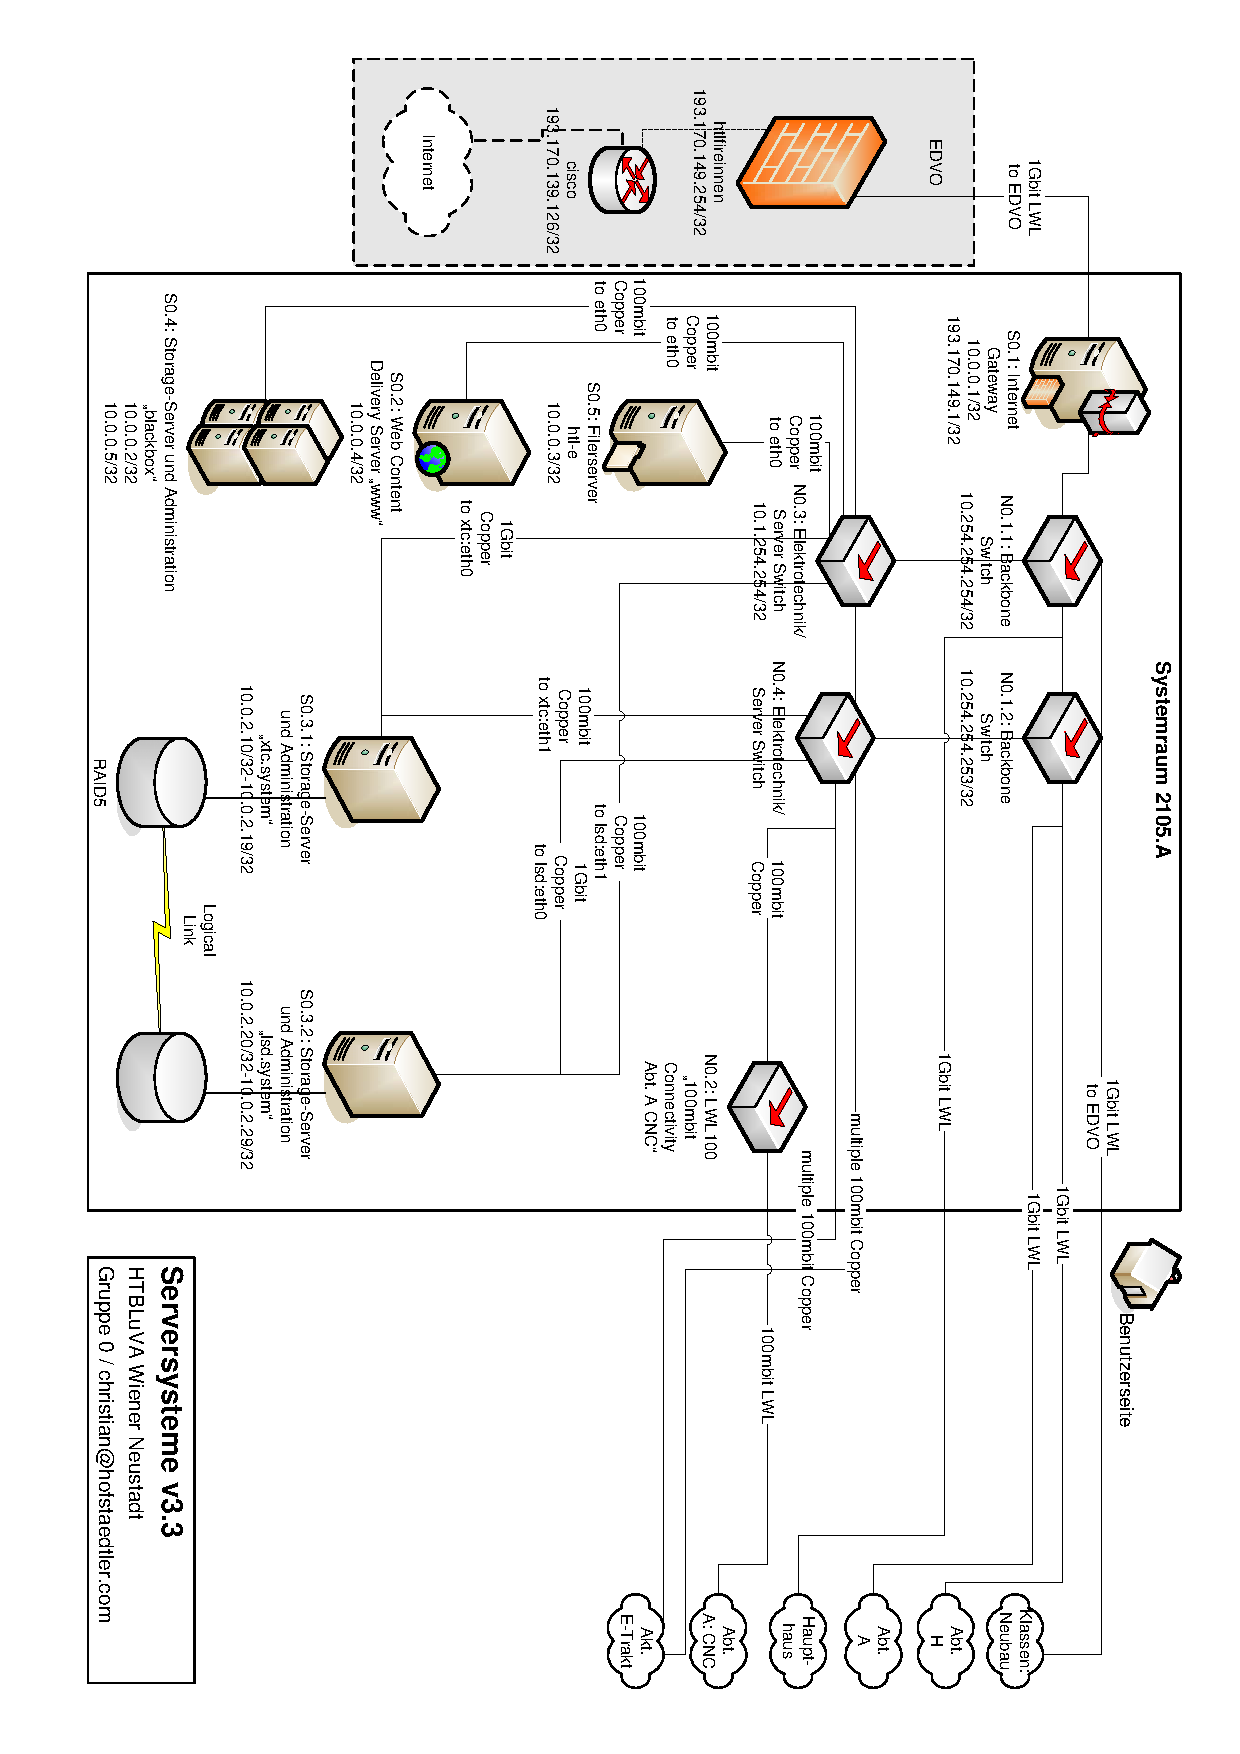
\includepdf[pages={1}]{files/htl-net-struct.pdf}
%\{htl-net-struct.pdf}{HTL Netzwerkstruktur}

\cChapter{HTL eDirectory Struktur}
\begin{landscape}
Im folgenden findet sich eine �bersicht des eDirectory Verzeichnisses. Hier mit Treename "HTL" und Basiskontext "o=htlwrn,c=at".

Der Kontext "o=System" ist nicht via LDAP sichtbar, kann daher auch nicht einfach von Applikationen ver�ndert/besch�digt werden.

\placefig{htl-nds-struct}{HTL eDirectory Struktur}

FIXME: Administration Container zeichnen.

\par

\section{Neue eDirectory Attribute}

inetStatus, loggedonHost, loggedonMac, traffic und lastActivity werden in den Benutzer-, Gruppen-, Klassen-, und Computer-Objekten verwendet. Die qbePolicy*-Attribute werden nur f�r die Computer-Policy-Objekte (qbeHostPolicy) verwendet.

\begin{lstlisting}
attributeTypes: ( 1.2.826.0.1.16224.0.0.0.10 NAME 'inetStatus' SYNTAX 1.3.6.1.4.1.1466.115.121.1.27 SINGLE-VALUE )
attributeTypes: ( 1.2.826.0.1.16224.0.0.0.11 NAME 'loggedonHost' SYNTAX 1.3.6.1.4.1.1466.115.121.1.15{64512} SINGLE-VALUE )
attributeTypes: ( 1.2.826.0.1.16224.0.0.0.12 NAME 'loggedonMac' SYNTAX 1.3.6.1.4.1.1466.115.121.1.15{128} SINGLE-VALUE )
attributeTypes: ( 1.2.826.0.1.16224.0.0.0.13 NAME 'traffic' SYNTAX 1.3.6.1.4.1.1466.115.121.1.36{64512} SINGLE-VALUE )
attributeTypes: ( 1.2.826.0.1.16224.0.0.0.14 NAME 'lastActivity' SYNTAX 1.3.6.1.4.1.1466.115.121.1.27 SINGLE-VALUE )
attributeTypes: ( 1.2.826.0.1.16224.0.0.0.15 NAME 'qbePolicyDynamicUserGroup' SYNTAX 1.3.6.1.4.1.1466.115.121.1.15{64512} )
attributeTypes: ( 1.2.826.0.1.16224.0.0.0.16 NAME 'qbePolicyDynamicUserEnabled' SYNTAX 1.3.6.1.4.1.1466.115.121.1.27 SINGLE-VALUE )
attributeTypes: ( 1.2.826.0.1.16224.0.0.0.17 NAME 'qbePolicyName' SYNTAX 1.3.6.1.4.1.1466.115.121.1.12 )
attributeTypes: ( 1.2.826.0.1.16224.0.0.0.18 NAME 'qbePolicyLoginScript' SYNTAX 1.3.6.1.4.1.1466.115.121.1.15{64512} SINGLE-VALUE )
attributeTypes: ( 1.2.826.0.1.16224.0.0.0.19 NAME 'qbePolicyHomeDrive' SYNTAX1.3.6.1.4.1.1466.115.121.1.15{64512} SINGLE-VALUE )
attributeTypes: ( 1.2.826.0.1.16224.0.0.0.20 NAME 'qbePolicyHomeDriveDir' SYNTAX 1.3.6.1.4.1.1466.115.121.1.15{64512} SINGLE-VALUE )
\end{lstlisting}

Bei einer Neuinstallation sollten die Attribute inetStatus, loggedonHost, loggedonMac, traffic und lastActivity auf qbe* umbenannt werden. Dies w�rde die Schemaverwaltung vereinfachen, zieht jedoch auch �nderungen in den PHP Skripten nach sich.


\section{Neue eDirectory Objekte}

qbeOrganizationalUnit und qbeGroup werden f�r die Klassen-/Gruppen-Verwaltung verwendet. qbeIpDevice, qbeOwnedObject und qbeHostPolicy f�r die ComputerVerwaltung.

\begin{lstlisting}
objectClasses: ( 1.2.826.0.1.16224.0.0.0.1 NAME 'qbeOrganizationalUnit' SUP organizationalUnit AUXILIARY MAY ( cn $ inetStatus ) X-NDS_NOT_CONTAINER '1' )
objectClasses: ( 1.2.826.0.1.16224.0.0.0.2 NAME 'qbeGroup' SUP groupOfNames AUXILIARY MAY inetStatus X-NDS_NOT_CONTAINER '1' )

objectClasses: ( 1.2.826.0.1.16224.0.0.0.3 NAME 'qbeIpDevice' AUXILIARY MAY ( macAddress $ ipHostNumber $ qbePolicyName ) X-NDS_NOT_CONTAINER '1' )
objectClasses: ( 1.2.826.0.1.16224.0.0.0.4 NAME 'qbeOwnedObject' AUXILIARY MAY owner X-NDS_NOT_CONTAINER '1' )
objectClasses: ( 1.2.826.0.1.16224.0.0.0.5 NAME 'qbeHostPolicy' AUXILIARY MUST qbePolicyDynamicUserEnabled MAY ( qbePolicyDynamicUserGroup $ qbePolicyHomeDrive $ qbePolicyHomeDriveDir $ qbePolicyLoginScript ) X-NDS_NOT_CONTAINER '1' )
\end{lstlisting}

\end{landscape}


\cChapter{Cluster-Installation HTL}

Der HTL-Cluster f�r den Authentication Server besteht aus zwei identischen Intel-Servern. Der Cluster-Name lautet auf qbe-auth.htlwrn.ac.at. Die Intel-Server wurden xtc.system.htlwrn.ac.at (Prim�rer Server) und lsd.system.htlwrn.ac.at (Sekund�rer Server) getauft.

Als Cluster Monitor-Software wird heartbeat eingesetzt. Die Intel-Server sind vom Modell SR2300 und mit dem Intel SE7501WV2 sowie dem Intel Raid-Controller SRCZCR ausgestattet.

Novell eDirectory wird nicht vom heartbeat verwaltet, es l�uft immer auf beiden Cluster Nodes. Alle anderen Dienste werden vom heartbeat gestartet/gestoppt.

Die Cluster-Applikationen und IP-Adressen:
\begin{description}
\item[Filesystem::/dev/nb0::/raid::ext3::noatime,usrquota,grpquota]{Das /raid (Daten-)Dateisystem}
\item[qbe-sas-daemon]{Hintergrunddienste vom Application Server}
\item[10.0.2.100]{Application Server IP}
\item[172.16.0.1/16]{Application Server IP f�r unbekannte Clients}
\item[apache::/etc/apache/httpd.conf]{Application Server Webserver}
\item[samba]{CIFS Server}
\item[mysql]{SQL Server}
\item[vsftpd]{FTP Server}
\item[nfs-kernel-server]{Network File System (NFS) Server f�r die www}
\item[dhcp3-server]{DHCP Server}
\item[10.0.2.104]{SubVersion IP}
\item[apache2]{SubVersion Server}
\end{description}


%% *eof*


%%
%% Qbe SAS SystemDocumentation
%% (C) Copyright 2001-2004 Christian Hofstaedtler
%%
%% $Id: part-last.tex 16 2004-04-30 12:55:13Z ch $
%%

\cChapter{T�tigkeitsprotokoll}

Dies ist die m�glicherweise unvollst�ndige Auflistung der T�tigkeiten, beginnend mit dem 31. Oktober 2003 -- also kurz nach der Umstellung auf die neuen Intel Server.
Arbeiten vor diesem Datum sind nicht mehr in der Liste, und wurden auch nirgends richtig dokumentiert. Die Arbeiten w�ren z.B. Erstellung des LDAP Baumes, Import der Benutzer, Kampf mit dem OpenLDAP Server, Beginn des Web-Interfaces und Erstellung des Qbe SAS Clients in C.

\begin{longtable}{l|p{9.5cm}}
2004-04-29 & fixing design of /login/ (download page) \\
2004-04-29 & fixing bug with IE6 + /login/update.php showing download box twice \\
2004-04-29 & making changelog private \\
2004-04-17 & rewrote 90\% of computer administration \\
2004-04-17 & fixed the sql errors btw \\
2004-04-16 & todo: fix sum in filexs/index \\
2004-04-16 & fixed a bunch o' bugs in client + gina \\
2004-04-16 & released 2.23.89 today \\
2004-04-16 & some fixes to webinterface \\
2004-04-16 & readability fixes to sas.inc.php (mac etc) \\
2004-04-16 & 0.96-pre has arrived! \\
2004-04-15 & bugfix user import \\
2004-03-18 & sas client 2.23.14 released: lots of bugfixes, auto logon to qbe-auth as requested by CZ \\
2004-03-17 & style + security fixes \\
2004-03-17 & infosys link now points to /modules/infosys, lets see... \\
2004-03-17 & merged workstation add into normal computer add \\
2004-03-17 & released new qbesasclient+unix version, with new .net qbeservice \\
2004-03-16 & ported qbesvc over to .net the last few days... this should get us: no more crashes on windows, and linux (macos?) support! \\
2004-03-09 & removed login/ssl links from logged-out menu, we have an ssl loginbox anyway \\
2004-03-08 & ok changed background color to blue again \\
2004-03-08 & added infosys module per request \\
2004-03-08 & fixed filexs group permission bug \\
2004-03-08 & fixed filexs xfer-put problems \\
2004-03-06 & adding in ldap call result caching \\
2004-03-06 & switched to xhtml 1.0, hopefully valid... \\
2004-03-06 & switched to new stylesheet \\
2004-03-06 & turned off iframe support in modules/redir/outside.php \\
2004-03-05 & reinstalled status with fz \\
2004-03-05 & adding in more macaddress validity checks \\
2004-03-05 & iis is now fixed \\
2004-03-05 & hm some users are reporting qbesvc crashes again, again in ntdll... \\
2004-03-01 & fixed lots of stuff in sasclient, uploaded 2.23.04 \\
2004-03-01 & added new "development patches" list to clientupdate page, added second version that wont autoupdate... \\
2004-03-01 & broke IE's webmail view somehow with strict mode, dunno why it doesnt want the iframe \\
2004-02-29 & fixed redirect to localservername instead of globalservername in checklogin, moved globalservername config to defines.app.php \\
2004-02-29 & ssl seems to work now without problems \\
2004-02-29 & added sidebar login form if not logged in \\
2004-02-29 & switched to standards compliance mode, hope this makes no further problems \\
2004-02-27 & fixed lots of permission problems in the webinterface \\
2004-02-27 & added "reown" for clients \\
2004-02-26 & ilogin update to 2.23.01, fixing some startup problems \\
2004-02-26 & added new "groups" share to samba, this is /export/groups, as in the filexs module \\
2004-02-26 & changed manage-objects/display-user from post to get, fixing the broken link when saving the userobject \\
2004-02-26 & moved sendmsg from menu to manage-objects \\
2004-02-26 & updates in addclient\_nt \\
2004-02-26 & fixing bugs in groupeditor \\
2004-02-21 & bugfixing in sasclient the whole day... \\
2004-02-21 & 00:34 - 90\% of new protocol description in manual done...tired... \\
2004-02-21 & fixed cb's typo 'Verwalteng' \\
2004-02-21 & btw, made some cool new issue's yesterday \\
2004-02-21 & got lots of complaints of broken links in the webinterface, will fix them now or then. \\
2004-02-16 & added more diag to failures in qbe-appmodule-ilogin-rpclogin \\
2004-02-13 & fixed bug with sysinfo \\
2004-02-13 & fixed bug with filexs not able to do anything \\
2004-02-11 & fixed some bugs in group editor \\
2004-02-11 & thought about lib for search blah \\
2004-02-11 & fixed bug in time display on every page \\
2004-02-11 & now worked 4h with teh web interface, no ssl errors... hopefully it works now \\
2004-02-11 & fixed webmail link \\
2004-02-11 & added a few lib functions, dont like to doc them atm. \\
2004-02-11 & added redpill into / and htaccess, so if you have a server downtime, just use the htaccess haha \\
2004-02-11 & added class lookup provider, not fully working \\
2004-02-11 & moved inetsave log to sql \\
2004-02-11 & added "last inet lock opener" to internet module \\
2004-02-11 & added "magic edvo user import on logon" for infothek-ips \\
2004-02-10 & hopefully fixed ssl problems (2) \\
2004-02-10 & added pc delete page \\
2004-02-10 & redid some tables \\
2004-02-10 & moved user,group,class management into the user manager \\
2004-02-10 & created new object manager \\
2004-02-10 & enhanced reporter \\
2004-02-10 & fixed some bugs in class editor \\
2004-02-09 & last week: did ilogin things... \\
2004-02-09 & debugging ssl problems... \\
2004-02-09 & hopefully fixed ssl problems \\
2004-01-30 & released client 2.22.00 (gold master), with a lot of fixes to the installer, service, tray, new gina, etc \\
2004-01-30 & held meeting with fz and sc about edvo-users \\
2004-01-30 & started coding of edvo-integration for "infothek" \\
2004-01-27 & done new sasgina today+yesterday... well it works \\
2004-01-24 & 02:10AM: wrote qbe\_ldap\_checkuser in C(++) using winldap calls... what a mess... * ch went to bed. \\
2004-01-23 & updated docs \\
2004-01-23 & updated ilogin to 2.21.03 \\
2004-01-22 & fixed ftp/passive problems \\
2004-01-22 & added internet/stats-traffic-iprange yesterday, completed it today \\
2004-01-22 & reconfigured network-raid, now syncs completly in 3h \\
2004-01-22 & added rsync for /qbe, xtc is master, lsd slave \\
2004-01-19 & merged /qbe/sysstate into /qbe/status/acl, removed dyna-acl which caused a lot of problems in the past \\
2004-01-18 & updated colors \\
2004-01-18 & removed network image from frontpage \\
2004-01-18 & fixed error if qbe\_app\_frontpage was empty \\
2004-01-18 & removed image from login form, form didnt look good if image wasnt there cause of X reasons \\
2004-01-18 & renamed login to Anmelden to make it consistent with the rest \\
2004-01-17 & fixed inetstatus save bug in modules/ldap/save-user.php, thanks to clemens+co \\
2004-01-15 & gestern: 19:00-00:30 uhr: gateway mit debian neu aufgesetzt, konfiguriert \\
2004-01-15 & ldap auth, squid, websense auf egw fertig konfiguriert \\
2004-01-09 & fixed things on status (mrtg etc) \\
2004-01-08 & fixed bug in ldif/import* \\
2004-01-08 & looked up realtek data sheets \\
2004-01-07 & fixed bug in checkaclupdate for proxy \\
2004-01-04 & 02:43 comitting: removed lots of old files, still writing docupdates \\
2004-01-04 & 03:51 uploaded new docpdf, gone sleeping \\
2003-12-28 & 20,21,22,23,25,27: documentation updates \\
2003-12-28 & fixed userlookup popup form \\
2003-12-28 & wrote a demo module, see /modules/dev/demo \\
2003-12-28 & added pretty print (table) to the changelog module \\
2003-12-28 & increased version to 0.9.2-alpha \\
2003-12-28 & corrected 193.170.149.2 mapping to status.htlwrn.ac.at \\
2003-12-19 & fixed filexs \\
2003-12-18 & added christmas special for ilogin2 \\
2003-12-18 & fixed zone htlwrn.ac.at on xtc dns and added flashlight \\
2003-12-18 & hopefully fixed problems with auto-dhcp clients (bound 172.16.0.1 ip etc) \\
2003-12-18 & fixed unreachable services from outside caused by alias/ip-change of blackbox.htlwrn.ac.at \\
2003-12-16 & modified statistics/systeminfo to look better etc \\
2003-12-15 & updated ilogin to 2.21.01 \\
2003-12-10 & moved a lot from /admin/admin/ to /modules/(core|ldap|ldif)/ \\
2003-12-10 & added /modules/core/sendmsg \\
2003-12-10 & completed menu restructure, changed core and ldap/user defines \\
2003-12-10 & added the "providers" system for module capabilities \\
2003-12-10 & added a popup for user lookup, doesnt work completely \\
2003-12-09 & fixed client pc self-add for users \\
2003-12-09 & modified sas\_ldap\_getusername() to accept dn's also \\
2003-12-02 & made a lot of changes to ilogin \\
2003-12-02 & moved a lot of files from /admin/ to /modules/(internet|core) \\
2003-12-02 & fixed internet stats links \\
2003-11-26 & turned off clustering for now \\
2003-11-26 & removed drbd, added dhcp and apache correctly to heartbeat, /dev/sda7 now gets mounted under /raid not /data \\
2003-11-26 & reconfigured fstabs on the other server so that nfs will work better after server failure \\
2003-11-26 & added logging facility (syslog) to a lot of phps \\
2003-11-24 & restarted xtc due to server hangup \\
2003-11-24 & added rfid module \\
2003-11-22 & restructured directory usage, added /modules/ and dynamic menu creation \\
2003-11-22 & completed filexs system level helper rewrite \\
2003-11-22 & created some debian qbe packages... \\
2003-11-21 & (ch) fixed user auto deletion from IE \\
2003-11-20 & readded focus() in loginform \\
2003-11-20 & started filexs-system part rewrite \\
2003-11-19 & readded missing features \\
2003-11-19 & added upload for filexs \\
2003-11-19 & started importer interface \\
2003-11-18 & completed reports interface \\
2003-11-18 & updated changelog interface \\
2003-11-18 & added filexs \\
2003-11-16 & updated complete layout \\
2003-11-16 & fixed mysql \\
2003-11-16 & found why qbelog.pl got started so often through cron \\
2003-11-03 & fixed a lot of problems after move to xtc \\
2003-10-31 & got nss\_ldap on xtc working against edirectory \\
\end{longtable}

%% *eof*



\newpage
\printindex

\end{document}

%% *eof*
